\documentclass[12pt,a4paper]{article}
\usepackage[a4paper, margin=0.8in, headheight=14pt]{geometry}
\usepackage{fontspec}
\usepackage{unicode-math}
\setmainfont{TeX Gyre Pagella}
\setmonofont[Scale=0.88]{TeX Gyre Cursor}
\setmathfont{Latin Modern Math}
\usepackage{xcolor}
\usepackage{colortbl}
\usepackage{titlesec}
\usepackage{enumitem}
\usepackage{tabularx}
\usepackage{booktabs}
\usepackage{array}
\usepackage{amsmath}
\allowdisplaybreaks
\usepackage{tikz}
\usetikzlibrary{shapes.geometric, arrows.meta, positioning, calc, fit, decorations.pathreplacing, decorations.pathmorphing, patterns, backgrounds}
% circuitikz not required for this subject
\usepackage{tcolorbox}
\tcbuselibrary{skins, breakable}
\usepackage{etoolbox}
\usepackage{hyperref}
\usepackage{fancyhdr}
\usepackage{graphicx}
\usepackage{microtype}
\hyphenpenalty=10000
\exhyphenpenalty=10000
\sloppy
\usepackage{caption}
\usepackage{setspace}
\usepackage{multirow}
\usepackage{tocloft}
\newcommand{\Q}[1]{\textbf{#1}\par\noindent\ignorespaces}
\definecolor{myred}{RGB}{196,30,58}
\definecolor{mydark}{RGB}{30,30,50}
\definecolor{mygreen}{RGB}{14,120,80}
\definecolor{myteal}{RGB}{0,130,140}
\definecolor{myamber}{RGB}{180,100,0}
\definecolor{mypurple}{RGB}{100,30,160}
\definecolor{mygray}{RGB}{246,247,249}
\definecolor{mgframe}{RGB}{180,185,200}
\definecolor{watermark}{RGB}{145,150,170}
\definecolor{hdrred}{RGB}{250,232,235}
\definecolor{hdrgreen}{RGB}{220,244,233}
\definecolor{hdrteal}{RGB}{220,242,244}
\definecolor{hdramber}{RGB}{253,242,215}
\definecolor{hdrpurple}{RGB}{238,228,255}
\definecolor{hdrgray}{RGB}{238,240,245}
\definecolor{rowalt}{RGB}{250,251,253}
\AfterEndEnvironment{tcolorbox}{\color{mydark}}

\titleformat{\section}{\large\bfseries\color{myred}}{\thesection.}{0.5em}{}[\vspace{1pt}{\color{myred}\rule{\linewidth}{0.8pt}}]
\titleformat{\subsection}{\normalsize\bfseries\color{myteal}}{\thesubsection}{0.5em}{}
\titlespacing*{\section}{0pt}{18pt}{7pt}
\titlespacing*{\subsection}{0pt}{11pt}{4pt}
\setlength{\parindent}{0pt}
\setlength{\parskip}{4pt}
\renewcommand{\cfttoctitlefont}{\large\bfseries\color{myred}}
\renewcommand{\cftaftertoctitle}{\par\noindent{\color{myred}\rule{\linewidth}{0.8pt}}}
\setlength{\cftbeforetoctitleskip}{0pt}
\setlength{\cftaftertoctitleskip}{6pt}
\renewcommand{\cftsecfont}{\normalsize\bfseries\color{mydark}}
\renewcommand{\cftsecpagefont}{\normalsize\bfseries\color{mydark}}
\renewcommand{\cftsecleader}{\cftdotfill{\cftdotsep}}
\setlength{\cftbeforesecskip}{7pt}
\renewcommand{\cftsubsecfont}{\small\color{mydark}}
\renewcommand{\cftsubsecpagefont}{\small\color{mydark}}
\setlength{\cftbeforesubsecskip}{3pt}
\setlength{\cftsubsecindent}{1.4em}
\renewcommand{\cftpartfont}{\normalsize\bfseries\color{myteal}}
\renewcommand{\cftpartpagefont}{\normalsize\bfseries\color{myteal}}
\setlength{\cftbeforepartskip}{14pt}
\renewcommand{\arraystretch}{1.45}
\setlength{\tabcolsep}{6pt}
\arrayrulecolor{mydark}
\newcolumntype{B}[1]{>{\small\bfseries\raggedright\arraybackslash}m{#1}}
\newcolumntype{C}[1]{>{\centering\arraybackslash}m{#1}}
\newcolumntype{Y}{>{\small\raggedright\arraybackslash}X}
\renewcommand{\tabularxcolumn}[1]{m{#1}}
\newcommand{\currmodule}{Module 1}
\pagestyle{fancy}
\fancyhf{}
\fancyhead[L]{\small\color{myred}\textbf{26-ES-EE101}\;\color{mydark}--- Basic Electrical and Electronics Engineering}
\fancyhead[R]{\small\color{myteal}\textbf{\currmodule\ Notes}}
\fancyfoot[C]{\small\color{mydark}\thepage}
\fancyfoot[R]{\small\color{watermark}\textit{\copyright\ Biraj}}
\renewcommand{\headrulewidth}{0.5pt}
\renewcommand{\footrulewidth}{0.3pt}

\hypersetup{colorlinks=true, linkcolor=myteal, urlcolor=myteal,
  pdfauthor={Biraj Sarkar},
  pdftitle={26-ES-EE101 --- Combined Notes}}

\tcbset{
  tikzbox/.style={
    colback=mygray, colframe=mgframe, boxrule=0.6pt, arc=4pt,
    left=8pt, right=8pt, top=6pt, bottom=6pt,
    colbacktitle=mgframe, coltitle=mydark, fonttitle=\small\bfseries
  },
  defbox/.style={
    colback=hdrgreen, colframe=mygreen, boxrule=0.8pt, arc=4pt,
    left=9pt, right=9pt, top=6pt, bottom=6pt,
    colbacktitle=mygreen, coltitle=white, fonttitle=\small\bfseries
  },
  formulabox/.style={
    colback=hdrteal, colframe=myteal, boxrule=0.8pt, arc=4pt,
    left=9pt, right=9pt, top=7pt, bottom=7pt,
    colbacktitle=myteal, coltitle=white, fonttitle=\small\bfseries
  },
  examplebox/.style={
    colback=hdramber, colframe=myamber, boxrule=0.8pt, arc=4pt,
    left=9pt, right=9pt, top=6pt, bottom=6pt,
    colbacktitle=myamber, coltitle=white, fonttitle=\small\bfseries
  },
  masonbox/.style={
    colback=hdrpurple, colframe=mypurple, boxrule=0.8pt, arc=4pt,
    left=9pt, right=9pt, top=6pt, bottom=6pt,
    colbacktitle=mypurple, coltitle=white, fonttitle=\small\bfseries
  },
  exambox/.style={
    colback=hdrpurple, colframe=mypurple, boxrule=1pt, arc=5pt,
    left=10pt, right=10pt, top=8pt, bottom=8pt,
    colbacktitle=mypurple, coltitle=white, fonttitle=\bfseries,
    breakable, title after break={\textbf{Frequently Asked / Viva Questions (contd.)}}
  }
}
\tcbset{breakable}
\tcbset{coltext=mydark}
\tcbset{after={\color{mydark}}}

\tikzset{
  block/.style={rectangle, draw=myteal, fill=hdrteal,
    text width=2.4cm, align=center, minimum height=0.95cm,
    font=\small, rounded corners=3pt, line width=0.7pt},
  redblock/.style={rectangle, draw=myred, fill=hdrred,
    text width=2.4cm, align=center, minimum height=0.95cm,
    font=\small, rounded corners=3pt, line width=0.7pt},
  sumjunc/.style={circle, draw=myamber, fill=hdramber,
    minimum size=0.62cm, font=\small, line width=0.8pt},
  arrow/.style={-Stealth, thick, color=mydark},
  redarrow/.style={-Stealth, thick, color=myred},
  line/.style={thick, color=mydark}
}

\newcommand{\modulestart}[2]{%
  \clearpage
  \renewcommand{\currmodule}{Module #1}%
  \renewcommand{\theHsection}{mod#1.\arabic{section}}%
  \renewcommand{\theHsubsection}{\theHsection.\arabic{subsection}}%
  \renewcommand{\theHsubsubsection}{\theHsubsection.\arabic{subsubsection}}%
  \phantomsection
  \addcontentsline{toc}{part}{Module #1: #2}%
  \setcounter{section}{0}%
  \begin{center}
    \vspace*{1.0cm}
    {\Huge\bfseries\color{myred} Module #1}\\[10pt]
    {\Large\bfseries\color{mydark} #2}\\[10pt]
    {\color{myred}\rule{0.55\linewidth}{1.2pt}}
  \end{center}
  \vspace{14pt}
}
\begin{document}

\thispagestyle{empty}

% ─── Page Border (TikZ Overlay) ────────────────────────────────────────────────
\begin{tikzpicture}[remember picture, overlay]
  % Outer border (fine line in mgframe)
  \draw[color=mgframe, line width=1.5pt] 
    ($(current page.north west) + (0.6in, -0.6in)$) rectangle 
    ($(current page.south east) + (-0.6in, 0.6in)$);
  % Inner border (finer accent line in myred)
  \draw[color=myred, line width=0.8pt] 
    ($(current page.north west) + (0.65in, -0.65in)$) rectangle 
    ($(current page.south east) + (-0.65in, 0.65in)$);
\end{tikzpicture}

\vspace*{1.0cm}
\begin{center}
  {\Huge\bfseries\color{myred} 26-ES-EE101}\\[10pt]
  {\LARGE\bfseries\color{mydark} Basic Electrical and Electronics Engineering}\\[20pt]
  {\color{myred}\rule{0.7\linewidth}{1.5pt}}\\[18pt]
  {\Large\color{myteal}\textbf{Combined Module Notes}}\\[8pt]
  {\large\color{mydark} Modules 1 -- 6}\\[40pt]
  {\normalsize\color{mydark} Semester I \quad$\bullet$\quad ECE \quad$\bullet$\quad 4 Credits}\\[12pt]
  {\normalsize\color{mydark} CGEC \;$|$\; MAKAUT Syllabus (A.Y. 2026--27)}
\end{center}
\vspace{1.0cm}
\begin{center}
  \begin{tcolorbox}[colback=mygray, colframe=mgframe, boxrule=0.5pt, arc=3pt, width=0.85\linewidth]
    \centering\small\color{mydark}
    \textbf{Disclaimer / Study Guide Notice:}\\
    These are condensed \textbf{Short Notes} focusing on core theory, key formulas, block/circuit diagrams, and standard viva Q\&As for university exam revision. Exhaustive numerical practice problems and derivation edge cases are not covered. This serves as a quick-revision reference guide for students.
  \end{tcolorbox}
\end{center}
\vfill
\vspace{0.6cm}
\begin{center}
  {\large\bfseries\color{mypurple} Biraj Sarkar}\\[16pt]
  {\footnotesize\color{watermark}\textbf{IN ASSOCIATION WITH}}\\[8pt]
  {\small\bfseries\color{mydark} MAKAUT Wingman \quad$\bullet$\quad MAKAUT Future Minds}\\[12pt]
  {\large\bfseries\color{myteal} Cooch Behar Government Engineering College}
\end{center}
\vfill
\begin{center}{\small\color{watermark}\textit{Exam-Ready Notes}}\end{center}
\clearpage

\hypersetup{linkcolor=mydark}
\tableofcontents
\hypersetup{linkcolor=myteal}
\clearpage

% -- Module 1 -----------------------------------------------------------------
\modulestart{1}{Basics of Electrical Wiring and Safety}

\section{Basics of Electrical Wiring and Safety}

\subsection{Electric shock and earthing}

\begin{tcolorbox}[defbox,title={Electric shock and protective earthing}]
Electric shock is the harmful effect of current passing through the body. Protective earthing connects exposed conductive parts, such as a metal appliance enclosure, to the protective earth system.
\end{tcolorbox}

\begin{itemize}[leftmargin=*, itemsep=3pt, topsep=4pt]
  \item \textbf{Effects.} Current through tissue can cause pain, muscle contraction, breathing difficulty, ventricular fibrillation and burns.
  \item \textbf{Severity.} It depends on current, duration, frequency, path and skin condition. A chest-crossing path is especially dangerous. Wet skin usually has a lower resistance.
  \item \textbf{Current estimate.} \(I=V/Z_{\mathrm{body}}\) explains the trend. Body impedance varies, so the estimate alone cannot establish a safe touch voltage.
\end{itemize}

\begin{itemize}[leftmargin=*, itemsep=3pt, topsep=4pt]
  \item \textbf{Normal condition.} Neutral carries the load return current. The protective-earth conductor carries negligible load current and serves a separate function downstream of the supply arrangement.
  \item \textbf{Fault on the case.} The earth bond gives fault current a return path, helps limit touch voltage and supports automatic disconnection.
  \item \textbf{Disconnection.} A fuse or breaker responds if the fault loop current is sufficient. A residual-current device (RCD) can respond to a much smaller leakage current.
\end{itemize}

\begin{tcolorbox}[tikzbox,title={Protective roles in a single-phase circuit},unbreakable]
\centering
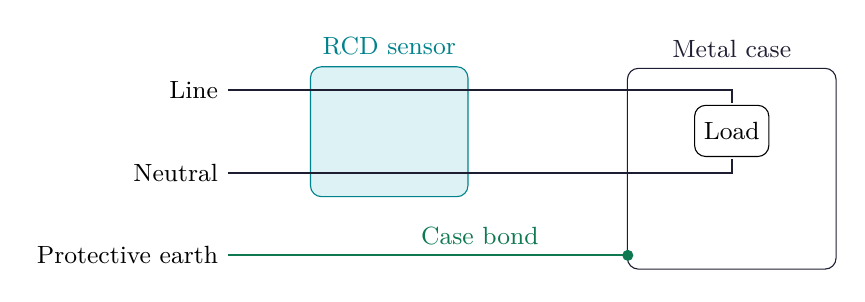
\begin{tikzpicture}[font=\small]
\node[left] at (0,2.2) {Line};
\node[left] at (0,1.15) {Neutral};
\node[left] at (0,0.1) {Protective earth};
\node[draw=myteal,fill=hdrteal,minimum width=2.0cm,minimum height=1.65cm,rounded corners] at (2.05,1.67) {};
\node[myteal,above] at (2.05,2.52) {RCD sensor};
\node[draw=mydark,minimum width=2.65cm,minimum height=2.55cm,rounded corners] (case) at (6.4,1.2) {};
\node[mydark,above] at (6.4,2.48) {Metal case};
\draw[line] (0,2.2)--(6.4,2.2)--(6.4,2.04);
\draw[line] (0,1.15)--(6.4,1.15)--(6.4,1.32);
\node[draw,rounded corners,fill=white,minimum height=0.65cm] at (6.4,1.68) {Load};
\draw[mygreen,thick] (0,0.1)--(5.08,0.1) node[pos=0.63,above] {Case bond};
\fill[mygreen] (5.08,0.1) circle (2pt);
\end{tikzpicture}
\end{tcolorbox}

For a shock incident, disconnect the supply safely before approaching the person, avoid direct contact while the supply may be live, and call emergency help. Repairs and inspection require isolation and verification by a competent person. In a written answer, state why earthing and automatic disconnection work together.

\subsection{Protective and switching devices}

\begin{itemize}[leftmargin=*, itemsep=3pt, topsep=4pt]
  \item \textbf{Overload.} Excessive current in a healthy circuit, often from too much connected load.
  \item \textbf{Short circuit.} Unintended low-impedance connection between points at different potentials.
  \item \textbf{Earth fault.} Unintended current from a live part to earth or to an earthed part.
\end{itemize}

An \textbf{RCD} detects the imbalance between currents in the live conductors passing through its sensor. In a healthy single-phase circuit the line and neutral currents cancel in the sensor. A leakage return outside the sensor gives a residual current:
\[
I_{\Delta}=\lvert I_L-I_N\rvert .
\]
An RCCB provides residual-current protection. An RCBO combines residual-current and overcurrent protection. A person touching line and neutral simultaneously may draw equal currents through both sensed conductors, so a residual-current device alone cannot be relied on in that case.

\par\vspace{6pt}\noindent
\begin{tabularx}{\linewidth}{|B{3.0cm}|Y|Y|}\hline
Device & \textbf{Working principle} & \textbf{Typical role} \\ \hline
SFU (switch-fuse unit) & A rated manual switch and fuse links. A link melts on excess current and is replaced after the fault is corrected. & Feeder isolation and overcurrent protection. \\ \hline
MCB (miniature circuit breaker) & Thermal action for overload and magnetic action for severe fault current in a typical thermal-magnetic design. Can be reset after clearing the fault. & Final-circuit overcurrent protection. \\ \hline
ELCB (earth leakage circuit breaker) & A traditional voltage-operated ELCB senses voltage rise on the protected earth system. The term is also used loosely for current-operated residual-current devices. & Earth-leakage protection. Identify the sensing principle explicitly in an answer. \\ \hline
MCCB (moulded-case circuit breaker) & A breaker for higher current or breaking-capacity duties, with thermal-magnetic or electronic trip depending on the design. & Distribution and industrial feeders. Some models offer adjustable settings. \\ \hline
\end{tabularx}

\begin{tcolorbox}[examplebox,title={Reading an RCD example}]
Suppose the line carries \(5.00\,\mathrm A\), and \(4.96\,\mathrm A\) returns through the sensed neutral.
\[
\begin{aligned}
I_\Delta &= \lvert 5.00-4.96\rvert\,\mathrm A\\
         &= 0.04\,\mathrm A\\
         &= 40\,\mathrm{mA}.
\end{aligned}
\]
This exceeds the \(30\,\mathrm{mA}\) rating of the device in this example. Actual disconnection depends on the RCD type and its operating conditions. The \(30\,\mathrm{mA}\) value is a device rating.
\end{tcolorbox}

\subsection{Wires, cables and Indian wiring practice}

A wire is an individual conductor, usually insulated where used in an installation. A cable is an assembly of one or more insulated conductors with any required sheath, screening or armour. Conductor cross-sectional area is expressed in \(\mathrm{mm^2}\). Copper and aluminium are common conductors. Stranding improves flexibility. PVC and XLPE are examples of insulation. A sheath protects against the environment, while armour provides mechanical protection when the service conditions require it.

Typical examples include solid or stranded single-core wires in conduit, multicore sheathed cables for fixed runs, flexible cords for movable appliances, and armoured cables for harsher routes. Selection depends on current capacity, permissible voltage drop, short-circuit withstand, mechanical duty, ambient temperature and grouping. The cable rating and the protection rating must be coordinated.

\begin{itemize}[leftmargin=*, itemsep=3pt, topsep=4pt]
  \item \textbf{Supply path.} Service connection, energy meter, main isolation, then distribution board and individual lighting and power circuits.
  \item \textbf{Distribution board.} Houses circuit protection and uses separate neutral and protective-earth connections as required by the earthing system.
  \item \textbf{Switch and outlet.} A switch or single-pole fuse in the line conductor interrupts the live feed. A three-pin outlet provides line, neutral and protective earth.
  \item \textbf{Wiring methods.} Conduit supports and protects conductors. Casing-and-capping and batten wiring are older methods.
\end{itemize}

Label line, neutral and protective earth as \(\mathrm{L}\), \(\mathrm{N}\) and \(\mathrm{PE}\). Common modern colours are brown, blue and green/yellow respectively. Verify each conductor's function because colours vary with age and standard. Before service, check earthing, polarity, continuity, insulation and protection.

\subsection{Batteries and their characteristics}

\begin{tcolorbox}[defbox,title={Cell, battery and capacity}]
A cell converts chemical energy to electrical energy. A battery contains one or more cells. Capacity (Ah) is the charge delivered under specified conditions.
\end{tcolorbox}

\begin{itemize}[leftmargin=*, itemsep=3pt, topsep=4pt]
  \item \textbf{Primary cells.} Intended for one discharge life. Alkaline cells are an example.
  \item \textbf{Secondary cells.} Rechargeable types include lead-acid (starting and backup), nickel-metal hydride and high-specific-energy lithium-ion. Use suitable charging and protection.
  \item \textbf{Compare cells by} voltage, capacity, energy, internal resistance, discharge rate, cycle life, self-discharge and charging needs. Capacity varies with load, temperature and cut-off voltage.
\end{itemize}

During discharge, \(V_t=E-Ir\), where \(E\) is open-circuit voltage and \(r\) is internal resistance. Matched cells add voltage in series and Ah in balanced parallel at the same voltage. A \(1C\) discharge current in amperes equals the capacity rating in Ah.

\begin{tcolorbox}[examplebox,title={Series battery rating and energy}]
Four \(3.2\,\mathrm V,\ 2\,\mathrm{Ah}\) cells in series retain \(Q_{\mathrm{pack}}=2\,\mathrm{Ah}\).
\[
\begin{aligned}
V_{\mathrm{pack}} &= 4(3.2)=12.8\,\mathrm V,\\
E_{\mathrm{nom}} &\approx V_{\mathrm{pack}}Q_{\mathrm{pack}}=12.8(2)=25.6\,\mathrm{Wh}.
\end{aligned}
\]
Ah measures charge. Wh measures energy (\(1\,\mathrm{Wh}=3600\,\mathrm J\)).
\end{tcolorbox}

\newpage
\begin{center}
  {\large\bfseries\color{myred} Quick Revision --- Module 1}\\[3pt]
  {\small\color{mydark} Basics of Electrical Wiring and Safety $|$ 26-ES-EE101}
\end{center}
\noindent{\color{myred}\rule{\linewidth}{1.2pt}}
\vspace{4pt}

\begin{tcolorbox}[formulabox, title={Key Formulas and Concepts at a Glance}]
\renewcommand{\arraystretch}{1.35}
\begin{tabularx}{\linewidth}{B{4.4cm}Y}
Residual current & $I_\Delta=\lvert I_L-I_N\rvert$ in A. \\[3pt]
Battery terminal voltage & $V_t=E-Ir$ during discharge. \\[3pt]
Nominal battery energy & $E_{\mathrm{nom}}\approx V_{\mathrm{nom}}Q$ in Wh for $Q$ in Ah. \\[3pt]
\end{tabularx}
\end{tcolorbox}

\begin{tcolorbox}[defbox, title={One-Line Definitions}]
\textbf{Protective earthing.} Bonding exposed conductive parts to the protective earth system.

\textbf{Breaking capacity.} Prospective fault current that a device can safely interrupt under its rated conditions.

\textbf{Self-discharge.} Loss of stored charge while a battery is idle.
\end{tcolorbox}

\begin{tcolorbox}[exambox, title={Frequently Asked / Viva Questions}]
\begin{enumerate}[topsep=0pt, label=\textbf{Q\arabic*.}, itemsep=5pt]
  \item \Q{What affects shock severity?} Current, duration, path, frequency and body conditions.
  \item \Q{Why earth a metal case?} The bond provides a fault path and supports fast disconnection.
  \item \Q{What does an RCD sense?} The nonzero sum of the currents in the monitored live conductors.
  \item \Q{Can an RCCB replace an MCB?} An RCCB covers residual current. The circuit also needs suitable overcurrent protection.
  \item \Q{How does an MCB distinguish overload and short circuit?} In the usual design a thermal element acts on sustained overload and a magnetic element acts rapidly on large fault current.
  \item \Q{What does SFU stand for?} Switch-fuse unit.
  \item \Q{What does armour do?} It gives mechanical protection to the cable.
  \item \Q{What is the role of a distribution board?} It divides the supply into final circuits and houses their protection.
  \item \Q{Which battery types can be recharged?} Secondary cells and batteries designed for repeated charge and discharge.
  \item \Q{What changes when matched cells are connected in series?} Voltages add and the ampere-hour capacity stays equal to that of one cell.
\end{enumerate}
\end{tcolorbox}

\begin{tcolorbox}[tikzbox, title={Summary Reference}]
\begin{tabularx}{\linewidth}{|B{4.0cm}|Y|}\hline
Topic & \textbf{What to remember} \\ \hline
Protection & Coordinate earthing, residual-current detection and overcurrent protection. \\ \hline
Wiring & Identify line, neutral and protective earth and state their separate functions. \\ \hline
Battery & State voltage and Ah separately and use Wh for energy. \\ \hline
\end{tabularx}
\end{tcolorbox}


% -- Module 2 -----------------------------------------------------------------
\modulestart{2}{Direct-Current Circuits}

\section{Direct-Current Circuits}

\subsection{Circuit elements, signs and sources}
\begin{tcolorbox}[defbox,title={Passive sign convention}]
Mark the reference current entering the terminal labelled positive. Then \(p=vi\) is the power absorbed. A negative result means the element delivers power. References remain fixed even if calculated signs are negative.
\end{tcolorbox}

With voltage in volts, current in amperes and time in seconds, \(1\,\Omega=1\,\mathrm{V/A}\). Element laws under the passive sign convention are
\[
\begin{aligned}
v_R&=Ri_R, & p_R&=Ri_R^2,\\
v_L&=L\,\frac{di_L}{dt}, & W_L&=\frac12 Li_L^2,\\
i_C&=C\,\frac{dv_C}{dt}, & W_C&=\frac12 Cv_C^2 .
\end{aligned}
\]
Inductance \(L\) is measured in henries, capacitance \(C\) in farads, power in watts and energy in joules. In settled DC with finite values an ideal inductor has zero voltage and an ideal capacitor has zero current. Resistances add in series. Conductances \(G=1/R\), in siemens, add in parallel.

An independent source imposes its stated voltage or current. A dependent source sets its output by a circuit voltage \(v_x\) or current \(i_x\). The four types are
\[
\begin{aligned}
v_s&=\mu v_x &&\text{voltage-controlled voltage source},\\
i_s&=g_m v_x &&\text{voltage-controlled current source},\\
v_s&=r_m i_x &&\text{current-controlled voltage source},\\
i_s&=\beta i_x &&\text{current-controlled current source}.
\end{aligned}
\]
The gains \(\mu,\beta\) are dimensionless, \(g_m\) is in S and \(r_m\) in \(\Omega\). The standard symbol has a diamond outline with a polarity mark or an arrow. In circuit analysis keep dependent sources active. A source transformation exchanges a voltage source \(V_s\) in series with \(R\) for a current source \(I_s=V_s/R\) in parallel with \(R\), preserving the external terminal behaviour and polarity.

\subsection{Kirchhoff's laws and systematic analysis}
\begin{tcolorbox}[defbox,title={KCL and KVL}]
Kirchhoff's current law (KCL) says the algebraic sum of currents at a node is zero, by charge conservation. Kirchhoff's voltage law (KVL) says the algebraic sum of voltage changes around a closed loop is zero in the lumped circuit model.
\end{tcolorbox}

\textbf{Nodal analysis} is efficient when there are few essential nodes.
\begin{enumerate}[leftmargin=*, itemsep=3pt, topsep=4pt]
  \item Choose a reference node and label the unknown node voltages.
  \item Write KCL using currents such as \((V_a-V_b)/R\) from \(a\) to \(b\).
  \item If a voltage source joins two unknown nodes, use a \textbf{supernode}. Write KCL at its outer boundary and add the source equation \(V_a-V_b=V_s\) for the stated polarity.
\end{enumerate}

\textbf{Mesh analysis} applies to planar circuits.
\begin{enumerate}[leftmargin=*, itemsep=3pt, topsep=4pt]
  \item Assign clockwise mesh currents and write KVL for each mesh.
  \item In mesh 1, a resistor shared with mesh 2 gives the drop \(R(I_1-I_2)\).
  \item If a current source is shared, use a \textbf{supermesh}: write KVL around its outside and add \(I_1-I_2=I_s\) when the source points in the mesh-1 direction.
\end{enumerate}

\begin{tcolorbox}[tikzbox,title={Two-mesh circuit with a shared resistor},unbreakable]
\centering
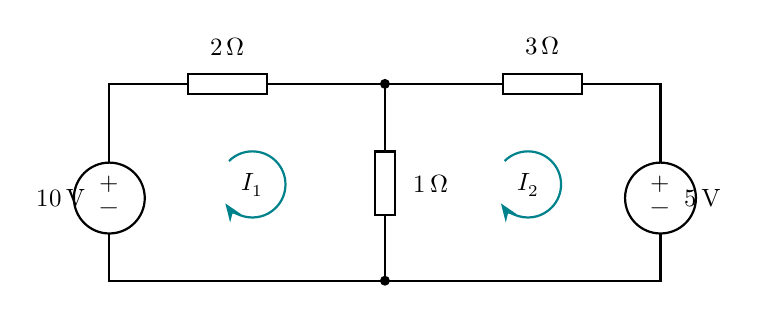
\begin{tikzpicture}[font=\small,line width=0.8pt]
\draw (0,1.5)--(0,2.5)--(1.0,2.5)
 (2.0,2.5)--(3.5,2.5)--(5.0,2.5)
 (6.0,2.5)--(7.0,2.5)--(7.0,1.5);
\draw (0,0.6)--(0,0)--(7.0,0)--(7.0,0.6);
\foreach \x/\volts/\side in {0/10/left,7/5/right}{
  \draw (\x,1.05) circle (0.45);
  \node at (\x,1.22) {$+$};
  \node at (\x,0.88) {$-$};
  \node[\side=5pt] at (\x,1.05) {$\volts\,\mathrm V$};
}
\draw (1.0,2.37) rectangle (2.0,2.63);
\draw (5.0,2.37) rectangle (6.0,2.63);
\node[above=3pt] at (1.5,2.63) {$2\,\Omega$};
\node[above=3pt] at (5.5,2.63) {$3\,\Omega$};
\draw (3.5,2.5)--(3.5,1.64) (3.5,0.83)--(3.5,0);
\draw (3.37,0.83) rectangle (3.63,1.64);
\node[right=3pt] at (3.63,1.23) {$1\,\Omega$};
\fill (3.5,2.5) circle (1.8pt) (3.5,0) circle (1.8pt);
\draw[-Stealth,myteal] (1.52,1.52) arc[start angle=135,end angle=-145,radius=0.42];
\node at (1.82,1.22) {$I_1$};
\draw[-Stealth,myteal] (5.02,1.52) arc[start angle=135,end angle=-145,radius=0.42];
\node at (5.32,1.22) {$I_2$};
\end{tikzpicture}
\end{tcolorbox}

\begin{tcolorbox}[examplebox,title={Find mesh currents and the shared-branch current}]
Take both top source terminals as positive and both mesh currents clockwise. Treat the source on the right as a \(5\,\mathrm V\) drop when traversed downwards.
\[
\begin{aligned}
2I_1+(I_1-I_2)&=10,\\
3I_2+(I_2-I_1)&=-5,\\
3I_1-I_2&=10,\qquad -I_1+4I_2=-5.
\end{aligned}
\]
\[
\begin{aligned}
I_2&=3I_1-10,\\
-I_1+4(3I_1-10)&=-5,\\
I_1&=\tfrac{35}{11}\,\mathrm A,\qquad I_2=-\tfrac{5}{11}\,\mathrm A,\\
I_{\mathrm{shared,down}}&=I_1-I_2=\tfrac{40}{11}\,\mathrm A.
\end{aligned}
\]
The right mesh current flows anticlockwise. Check by nodal analysis: the shared top node \(V\) satisfies
\[
\begin{aligned}
\tfrac{V-10}{2}+\tfrac{V-5}{3}+\tfrac{V}{1}&=0,\\
3(V-10)+2(V-5)+6V&=0,\\
V&=\tfrac{40}{11}\,\mathrm V.
\end{aligned}
\]
\end{tcolorbox}

\subsection{Star--delta transformation}
A star (Y) joins three arms \(R_a,R_b,R_c\) at an internal node. A delta (\(\Delta\)) joins the terminal pairs with resistances \(R_{ab},R_{bc},R_{ca}\). A transformation preserves resistance between any two terminals with the third terminal open. For example \(R_a+R_b=R_{ab}\parallel(R_{ca}+R_{bc})\). Write the two equivalent equations for the other pairs, add those involving terminal \(a\), subtract the remaining one, and divide by two to obtain the first formula below.

\begin{tcolorbox}[formulabox,title={Star--delta formulas}]
With \(S=R_{ab}+R_{bc}+R_{ca}\) and \(P=R_aR_b+R_bR_c+R_cR_a\),
\[
\begin{aligned}
R_a&=\frac{R_{ab}R_{ca}}{S},&
R_b&=\frac{R_{ab}R_{bc}}{S},&
R_c&=\frac{R_{bc}R_{ca}}{S},\\[3pt]
R_{ab}&=\frac{P}{R_c},&
R_{bc}&=\frac{P}{R_a},&
R_{ca}&=\frac{P}{R_b}.
\end{aligned}
\]
A balanced \(9\,\Omega\)-per-side delta becomes a \(3\,\Omega\)-per-arm star.
\end{tcolorbox}

\subsection{Superposition, Thevenin and Norton}
\begin{tcolorbox}[defbox,title={Three linear-network theorems}]
\textbf{Superposition.} A branch voltage or current in a linear circuit is the signed sum of the responses to each independent source acting alone.

\textbf{Thevenin.} A linear two-terminal circuit can be represented by an ideal voltage \(V_{\mathrm{th}}\) in series with \(R_{\mathrm{th}}\), when a finite Thevenin resistance exists.

\textbf{Norton.} The corresponding current-source model is \(I_{\mathrm N}\) in parallel with \(R_{\mathrm N}=R_{\mathrm{th}}\), when the Norton model is finite.
\end{tcolorbox}

\begin{itemize}[leftmargin=*, itemsep=3pt, topsep=4pt]
  \item \textbf{Superposition.} Short ideal independent voltage sources and open ideal independent current sources that are turned off. Keep dependent sources active. Sum signed voltage or current contributions before calculating power.
  \item \textbf{Thevenin voltage.} Disconnect the load and find the open-circuit voltage \(V_{\mathrm{oc}}\).
  \item \textbf{Port resistance.} Deactivate independent sources. With dependent sources present, drive the port with a test source and use \(R_{\mathrm{th}}=V_t/I_t\), with test current entering the port.
  \item \textbf{Norton current and cross-check.} \(I_{\mathrm N}=I_{\mathrm{sc}}\) supplied to an external short. If \(I_{\mathrm{sc}}\ne0\), \(R_{\mathrm{th}}=V_{\mathrm{oc}}/I_{\mathrm{sc}}\).
\end{itemize}

\begin{tcolorbox}[examplebox,title={From voltage divider to load power}]
A \(12\,\mathrm V\) source feeds a \(4\,\Omega\) series resistor and a \(6\,\Omega\) shunt resistor. The load is across the shunt.
\[
\begin{aligned}
V_{\mathrm{th}} &=12\frac{6}{4+6}=7.2\,\mathrm V,\\
R_{\mathrm{th}} &=4\parallel 6=\frac{4(6)}{4+6}=2.4\,\Omega,\\
I_{\mathrm N} &=\frac{7.2}{2.4}=3\,\mathrm A.
\end{aligned}
\]
For \(R_L=3.6\,\Omega\), \(I_L=7.2/(2.4+3.6)=1.2\,\mathrm A\).
The load power is \(I_L^2R_L=5.184\,\mathrm W\).
\end{tcolorbox}

\begin{tcolorbox}[examplebox,title={Superposition with voltage and current sources}]
A \(12\,\mathrm V\) source feeds a node through \(3\,\Omega\). A \(6\,\Omega\) resistor connects the node to ground. A \(1\,\mathrm A\) source injects current into the node from ground.
\[
\begin{aligned}
V^{(12\mathrm V)} &= 12\frac{6}{3+6}=8\,\mathrm V
     &&\text{(open the current source)},\\
V^{(1\mathrm A)} &=1(3\parallel6)=2\,\mathrm V
     &&\text{(short the voltage source)},\\
V&=8+2=10\,\mathrm V.
\end{aligned}
\]
Check KCL: \((10-12)/3+10/6-1=0\,\mathrm A\). Power in the \(6\,\Omega\) branch is \(10^2/6=16.67\,\mathrm W\) using the total voltage.
\end{tcolorbox}

\subsection{Maximum power transfer}
For a positive \(R_{\mathrm{th}}\) and a variable resistive load, the load receives maximum power at \(R_L=R_{\mathrm{th}}\):
\[
\begin{aligned}
P_L&=\frac{V_{\mathrm{th}}^2R_L}{(R_{\mathrm{th}}+R_L)^2},\\
\frac{dP_L}{dR_L}
 &= V_{\mathrm{th}}^2
   \frac{R_{\mathrm{th}}-R_L}{(R_{\mathrm{th}}+R_L)^3},\\
R_{L,\mathrm{opt}}&=R_{\mathrm{th}},&
P_{\max}&=\frac{V_{\mathrm{th}}^2}{4R_{\mathrm{th}}}.
\end{aligned}
\]
For nonzero source voltage the derivative changes from positive to negative. In the equivalent series circuit half the power is dissipated internally at this point. In the voltage-divider example the optimum is \(2.4\,\Omega\) and \(P_{\max}=5.4\,\mathrm W\).

\subsection{First-order RL and RC transients}
A \textbf{transient} is the temporary response after switching. Capacitor voltage and inductor current remain continuous for finite currents and voltages.
\begin{enumerate}[leftmargin=*, itemsep=3pt, topsep=4pt]
  \item Choose the state \(x=v_C\) or \(x=i_L\) and find \(x(0^+)=x(0^-)\) from the pre-switch circuit.
  \item Find \(x_\infty\) from the new DC circuit.
  \item Use the resistance \(R_{\mathrm{eq}}\) seen by the storage element after switching. Calculate \(\tau=R_{\mathrm{eq}}C\) for RC or \(\tau=L/R_{\mathrm{eq}}\) for RL, in seconds.
\end{enumerate}
\[
\begin{aligned}
\frac{dx}{dt}+\frac{x}{\tau}&=\frac{x_\infty}{\tau},\\
\frac{d}{dt}(x-x_\infty)&=-\frac{x-x_\infty}{\tau},\\
x(t)&=x_\infty+[x(0^+)-x_\infty]e^{-t/\tau}.
\end{aligned}
\]
The remaining difference from steady state at \(t=\tau\) is \(e^{-1}\) times the initial difference. After \(5\tau\) it is about \(0.67\%\).

\begin{tcolorbox}[tikzbox,title={Normalised first-order step responses},unbreakable]
\centering
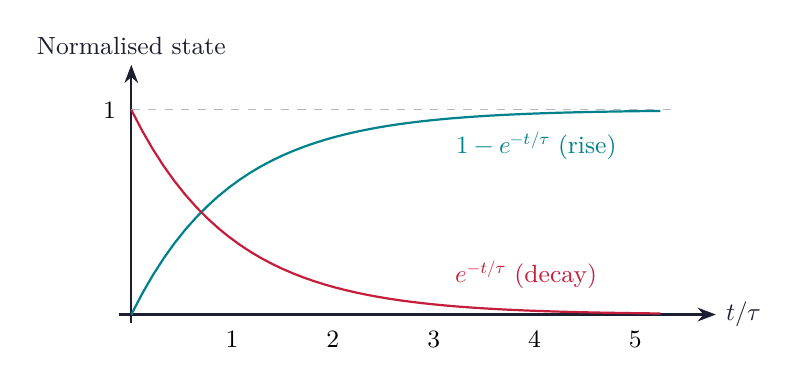
\begin{tikzpicture}[x=1.28cm,y=2.6cm,font=\small]
\draw[arrow] (-0.12,0)--(5.8,0) node[right] {$t/\tau$};
\draw[arrow] (0,-0.04)--(0,1.22) node[above] {Normalised state};
\draw[mgframe,dashed] (0,1)--(5.35,1);
\foreach \t in {1,2,3,4,5} \node[below] at (\t,-0.03) {\t};
\node[left=2pt] at (0,1) {1};
\draw[myteal,thick,domain=0:5.25,samples=50] plot (\x,{1-exp(-\x)});
\draw[myred,thick,domain=0:5.25,samples=50] plot (\x,{exp(-\x)});
\node[myteal,below] at (4.02,0.94) {$1-e^{-t/\tau}$ (rise)};
\node[myred,above] at (3.92,0.08) {$e^{-t/\tau}$ (decay)};
\end{tikzpicture}
\end{tcolorbox}

\begin{tcolorbox}[examplebox,title={Time constants and initial conditions},unbreakable]
An initially uncharged \(100\,\mu\mathrm F\) capacitor charges from \(10\,\mathrm V\) through \(2\,\mathrm{k}\Omega\).
\[
\begin{aligned}
\tau&=(2000)(100\times 10^{-6})=0.20\,\mathrm s,\\
v_C(t)&=10(1-e^{-t/0.20})\,\mathrm V,\\
v_C(0.20\,\mathrm s)&=6.32\,\mathrm V.
\end{aligned}
\]
For an RL step of \(12\,\mathrm V\), \(R=6\,\Omega\), \(L=3\,\mathrm H\), and \(i_L(0)=0\), the final current is \(2\,\mathrm A\) and \(\tau=0.50\,\mathrm s\). Thus \(i_L(t)=2(1-e^{-t/0.50})\,\mathrm A\).
\end{tcolorbox}

\newpage
\begin{center}
  {\large\bfseries\color{myred} Quick Revision --- Module 2}\\[3pt]
  {\small\color{mydark} Direct-Current Circuits $|$ 26-ES-EE101}
\end{center}
\noindent{\color{myred}\rule{\linewidth}{1.2pt}}
\vspace{4pt}

\begin{tcolorbox}[formulabox, title={Key Formulas and Concepts at a Glance}]
\renewcommand{\arraystretch}{1.35}
\begin{tabularx}{\linewidth}{B{4.4cm}Y}
Node current & $i_{ab}=(V_a-V_b)/R$ in A. \\[3pt]
Two-terminal equivalent & $V_{\mathrm{th}}=V_{\mathrm{oc}}$, $I_{\mathrm N}=I_{\mathrm{sc}}$. \\[3pt]
Maximum DC load power & $R_L=R_{\mathrm{th}}$, $P_{\max}=V_{\mathrm{th}}^2/(4R_{\mathrm{th}})$. \\[3pt]
Time constants & $\tau_{\mathrm{RC}}=RC$, $\tau_{\mathrm{RL}}=L/R$ in s. \\[3pt]
\end{tabularx}
\end{tcolorbox}

\begin{tcolorbox}[defbox, title={One-Line Definitions}]
\textbf{Mesh.} A loop in a planar circuit that encloses no smaller loop.

\textbf{Reference node.} The node assigned zero potential for the calculation.

\textbf{Time constant.} Time for the remaining first-order transient to fall to one over e of its initial value.
\end{tcolorbox}

\begin{tcolorbox}[exambox, title={Frequently Asked / Viva Questions}]
\begin{enumerate}[topsep=0pt, label=\textbf{Q\arabic*.}, itemsep=5pt]
  \item \Q{What physical principle gives KCL?} Conservation of charge at a node.
  \item \Q{What physical principle gives KVL?} A closed path has zero net voltage change in the lumped circuit model.
  \item \Q{When is a supernode used?} When an ideal voltage source joins two non-reference nodes.
  \item \Q{What makes a supermesh?} A current source lies on the boundary shared by two meshes.
  \item \Q{Can a dependent source be deactivated in superposition?} Keep its controlling relation active for each source contribution.
  \item \Q{Why superpose current before power?} Power is nonlinear in the branch current, for example $P=I^2R$.
  \item \Q{How do we find port resistance with a dependent source?} Turn off independent sources and apply a test source at the port.
  \item \Q{When is maximum power transferred to a resistive load?} When the positive load resistance equals the positive Thevenin resistance.
  \item \Q{Which two quantities are continuous at normal switching?} Inductor current and capacitor voltage.
  \item \Q{What are the settled DC models for L and C?} An ideal inductor is a short circuit and an ideal capacitor is an open circuit.
\end{enumerate}
\end{tcolorbox}

\begin{tcolorbox}[tikzbox, title={Summary Reference}]
\begin{tabularx}{\linewidth}{|B{4.0cm}|Y|}\hline
Topic & \textbf{What to remember} \\ \hline
Nodal method & Write KCL in terms of voltages and add source constraints. \\ \hline
Mesh method & Write KVL in terms of mesh currents and add current-source constraints. \\ \hline
Network equivalent & Remove the load, calculate port values, then reconnect the load. \\ \hline
\end{tabularx}
\end{tcolorbox}


% -- Module 3 -----------------------------------------------------------------
\modulestart{3}{Alternating-Current Circuits}

\section{Alternating-Current Circuits}

\subsection{Generation and measurement of AC}
\begin{tcolorbox}[defbox,title={Alternating voltage, period and RMS value}]
An alternating voltage changes polarity periodically. Its period \(T\) is the time for one cycle. Its root-mean-square (RMS) value equals the DC voltage that delivers the same average power to a given resistor.
\end{tcolorbox}

For \(N\) turns, uniform field \(B\) and coil area \(A\), the angle from the field to the coil normal is \(\omega t\). The flux per turn is \(BA\cos\omega t\). With the reference polarity set by Faraday's law,
\[
\begin{aligned}
v(t)&=-N\frac{d}{dt}(BA\cos\omega t)\\
    &=NBA\omega\sin\omega t
     =V_m\sin\omega t,\\
\omega&=2\pi f,\qquad T=\frac{1}{f}.
\end{aligned}
\]
Here \(f\) is in Hz, \(\omega\) in rad/s and \(V_m\) is the peak in volts. The signed cycle average of this sinusoid is zero. In form-factor calculations, use the average of the rectified waveform:
\[
\begin{aligned}
V_{\mathrm{av,rect}}
 &=\frac{1}{\pi}\int_0^\pi V_m\sin\theta\,d\theta
 =\frac{2V_m}{\pi},\\
V_{\mathrm{rms}}
 &=\sqrt{\frac{1}{2\pi}\int_0^{2\pi}V_m^2\sin^2\theta\,d\theta}
 =\frac{V_m}{\sqrt2},\\
\text{form factor}
 &=\frac{V_{\mathrm{rms}}}{V_{\mathrm{av,rect}}}=\frac{\pi}{2\sqrt2}\approx1.111,\\
\text{peak factor}
 &=\frac{V_m}{V_{\mathrm{rms}}}=\sqrt2.
\end{aligned}
\]
Use \(\sin^2\theta=(1-\cos2\theta)/2\) to evaluate the RMS integral. Apply the same definitions to current.

\subsection{Phasors and RLC circuits}
A phasor is a complex number representing the RMS magnitude and phase of a sinusoid at a fixed frequency. With cosine reference, \(v(t)=\sqrt2 V\cos(\omega t+\theta)\) corresponds to \(\underline V=V\angle\theta\). Compare phases only after expressing all quantities with the same frequency and sine or cosine reference.

\begin{itemize}[leftmargin=*, itemsep=3pt, topsep=4pt]
  \item \textbf{Impedance and admittance.} \(Z=\underline V/\underline I=R+jX\) is in \(\Omega\). \(Y=1/Z=G+jB_s\) is in S, with \(B_s\) the susceptance.
  \item \textbf{Resistor.} \(Z_R=R\). Current and voltage are in phase.
  \item \textbf{Inductor.} The derivative in \(v_L=L\,di_L/dt\) becomes \(j\omega\), so \(Z_L=j\omega L\). Current lags voltage by \(90^\circ\).
  \item \textbf{Capacitor.} From \(i_C=C\,dv_C/dt\), \(Z_C=1/(j\omega C)\). Current leads voltage by \(90^\circ\).
\end{itemize}

Add impedances in series and admittances in parallel:
\[
\begin{aligned}
Z_{\mathrm{series}}&=R+j\left(\omega L-\frac{1}{\omega C}\right),\\
Y_{\mathrm{parallel}}&=\frac{1}{R}
       +j\left(\omega C-\frac{1}{\omega L}\right).
\end{aligned}
\]
\begin{itemize}[leftmargin=*, itemsep=3pt, topsep=4pt]
  \item \textbf{Parallel branches.} The displayed expression assumes separate ideal \(R,L,C\) branches. In general, use \(Y_{\mathrm{in}}=\sum_k 1/Z_k\), then \(\underline I=\underline VY_{\mathrm{in}}\).
  \item \textbf{Series phasors.} With current as reference, \(V_R\) lies on the real axis, \(V_L\) points up and \(V_C\) points down. The net reactive voltage is \(I(X_L-X_C)\).
\end{itemize}

\begin{tcolorbox}[tikzbox,title={Series RLC phasors for a net inductive load},unbreakable]
\centering
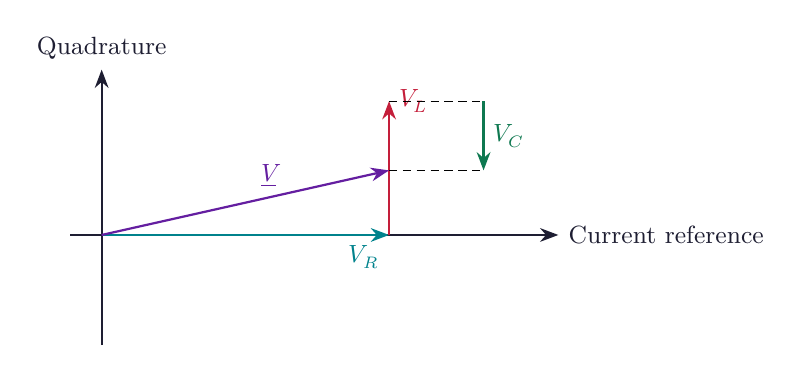
\begin{tikzpicture}[font=\small]
\draw[arrow] (-0.4,0)--(5.8,0) node[right] {Current reference};
\draw[arrow] (0,-1.4)--(0,2.1) node[above] {Quadrature};
\draw[arrow,myteal] (0,0)--(3.65,0) node[below left] {$V_R$};
\draw[arrow,myred] (3.65,0)--(3.65,1.7) node[right] {$V_L$};
\draw[arrow,mygreen] (4.85,1.7)--(4.85,0.82) node[midway,right] {$V_C$};
\draw[densely dashed] (3.65,1.7)--(4.85,1.7) (3.65,0.82)--(4.85,0.82);
\draw[arrow,mypurple] (0,0)--(3.65,0.82) node[pos=0.58,above] {$\underline V$};
\end{tikzpicture}
\end{tcolorbox}

\begin{tcolorbox}[examplebox,title={Solving a series RLC circuit}]
Apply \(100\angle0^\circ\,\mathrm V\) RMS to \(R=30\,\Omega\), \(X_L=60\,\Omega\), \(X_C=20\,\Omega\).
\[
\begin{aligned}
Z&=30+j40=50\angle53.13^\circ\,\Omega,\\
\underline I&=\frac{100\angle0^\circ}{50\angle53.13^\circ}\\
             &=2\angle(-53.13^\circ)\,\mathrm A.
\end{aligned}
\]
The lagging power factor is \(30/50=0.60\). The component voltage magnitudes are \(60\), \(120\) and \(40\,\mathrm V\). Their phasor sum has magnitude \(\sqrt{60^2+(120-40)^2}=100\,\mathrm V\).
\end{tcolorbox}

\begin{tcolorbox}[examplebox,title={Find the input of a parallel RLC circuit}]
For \(100\angle0^\circ\,\mathrm V\) RMS across separate \(R=50\,\Omega\), \(X_L=100\,\Omega\) and \(X_C=50\,\Omega\) branches,
\[
\begin{aligned}
Y&=\frac{1}{50}-j\frac{1}{100}+j\frac{1}{50}
  =0.020+j0.010\,\mathrm S,\\
\underline I&=100Y=2+j1\,\mathrm A,\\
Z&=\frac{1}{Y}=40-j20\,\Omega.
\end{aligned}
\]
Current leads voltage because the net susceptance is positive. The current magnitude is \(\sqrt5\,\mathrm A\).
\end{tcolorbox}

\subsection{Power and power-factor improvement}
\begin{tcolorbox}[defbox,title={Active, reactive and apparent power}]
Active power \(P\) is average energy delivered per second (W). Reactive power \(Q\) measures the quadrature part of the power exchange (var). Apparent power \(S\) is the product of RMS voltage and current (VA).
\end{tcolorbox}

Let \(\phi=\angle\underline V-\angle\underline I\). The product of the instantaneous sinusoids is \(VI[\cos\phi+\cos(2\omega t-\phi)]\) when \(v(t)=\sqrt2V\cos\omega t\). The double-frequency term averages to zero. Thus
\[
\begin{aligned}
\underline S&=\underline V\underline I^*=P+jQ,\\
P&=VI\cos\phi,& Q&=VI\sin\phi,\\
S&=VI=\sqrt{P^2+Q^2},& \mathrm{PF}&=P/S.
\end{aligned}
\]
Here \(Q>0\) for a net inductive load and \(Q<0\) for a net capacitive load. For sinusoidal passive loads the displacement power factor is \(\cos\phi\). In the series example \(P=120\,\mathrm W\), \(Q=160\,\mathrm{var}\), \(S=200\,\mathrm{VA}\).

\textbf{Procedure for correcting a lagging power factor.}
\begin{enumerate}[leftmargin=*, itemsep=3pt, topsep=4pt]
  \item Find the reactive demand before and after correction using \(Q=P\tan\phi\). Use the same active power \(P\).
  \item Select a shunt capacitor to supply \(Q_C=P(\tan\phi_1-\tan\phi_2)\), the difference between the old and target demands.
  \item For a single-phase supply, use \(C=Q_C/(\omega V^2)\) with RMS voltage \(V\). The supply current falls at the same active power because the source supplies less reactive current.
\end{enumerate}
At \(50\,\mathrm{Hz}\), cancelling the earlier \(160\,\mathrm{var}\) at \(100\,\mathrm V\) requires
\[
\begin{aligned}
C&=\frac{160}{2\pi(50)(100)^2}\,\mathrm F\\
 &=50.9\,\mu\mathrm F .
\end{aligned}
\]
In the ideal example supply current falls from \(2\,\mathrm A\) to \(1.2\,\mathrm A\); load-branch current is still \(2\,\mathrm A\).

\subsection{Series and parallel resonance}
Resonance means cancellation of the input reactive term at a particular frequency. In series RLC set \(X_L=X_C\). For parallel RLC with ideal reactive branches set their susceptances to cancel.
\[
\begin{aligned}
\omega_0 L &=\frac{1}{\omega_0 C},\\
f_0 &=\frac{1}{2\pi\sqrt{LC}}.
\end{aligned}
\]
\begin{itemize}[leftmargin=*, itemsep=3pt, topsep=4pt]
  \item \textbf{Series.} \(Z=R\) is minimum and the supply current is maximum at fixed voltage. The individual reactive voltages can be large. Quality factor is \(\omega_0L/R\).
  \item \textbf{Parallel.} With ideal \(L,C\) and \(R\) in separate branches, \(Y=1/R\) is minimum and supply current is minimum. The reactive branch currents can still be large. Coil resistance shifts the resonant frequency.
  \item \textbf{Numerical check.} \(L=0.1\,\mathrm H\) and \(C=100\,\mu\mathrm F\) give \(f_0\approx50.3\,\mathrm{Hz}\) in the ideal model.
\end{itemize}

\subsection{Balanced three-phase systems}
A balanced source has equal sinusoidal phase voltages spaced by \(120^\circ\). A balanced load presents equal phase impedances. In star, one end of each phase connects to the neutral point. The line voltage is the difference of two phase voltages. For a positive sequence,
\[
\begin{aligned}
\underline V_{AB}
 &= V_{\mathrm{ph}}\angle0^\circ-V_{\mathrm{ph}}\angle(-120^\circ)\\
 &=\sqrt3 V_{\mathrm{ph}}\angle30^\circ .
\end{aligned}
\]
Line current equals phase current in star. In delta the phases form a closed triangle so \(V_L=V_{\mathrm{ph}}\). A line current is a difference of two branch currents, for example \(\underline I_A=\underline I_{AB}-\underline I_{CA}\), so \(I_L=\sqrt3 I_{\mathrm{ph}}\) for a balanced delta.

\begin{tcolorbox}[formulabox,title={Balanced three-phase power}]
\[
\begin{aligned}
P_3&=3V_{\mathrm{ph}}I_{\mathrm{ph}}\cos\phi
    =\sqrt3 V_L I_L\cos\phi,\\
Q_3&=\sqrt3 V_L I_L\sin\phi,\qquad
S_3=\sqrt3 V_L I_L .
\end{aligned}
\]
\end{tcolorbox}

\textbf{Three-phase power measurement.}
For a three-wire load, place wattmeter current coils in lines A and B and use C as the common voltage-coil return. The meters sense \(V_{AC}\) with \(I_A\), and \(V_{BC}\) with \(I_B\). Since \(i_A+i_B+i_C=0\), the sum of the instantaneous meter products is
\[
(v_A-v_C)i_A+(v_B-v_C)i_B=v_Ai_A+v_Bi_B+v_Ci_C.
\]
The average therefore gives \(P_3=W_1+W_2\), including algebraic signs. In a balanced load, with the meters labelled so that \(W_1=V_L I_L\cos(30^\circ-\phi)\) and \(W_2=V_L I_L\cos(30^\circ+\phi)\),
\[
\tan\phi=\sqrt3\frac{W_1-W_2}{W_1+W_2}.
\]
A lagging angle above \(60^\circ\) gives a negative \(W_2\) in this labelling. In a four-wire load, one wattmeter per phase can give the total by summation. 
\begin{tcolorbox}[examplebox,title={Balanced star load and wattmeter readings}]
Take \(V_L=400\,\mathrm V\) and \(Z_{\mathrm{ph}}=20\angle36.87^\circ\,\Omega\).
\[
\begin{aligned}
V_{\mathrm{ph}}&=\frac{400}{\sqrt3}=230.94\,\mathrm V,\\
I_L&=I_{\mathrm{ph}}=\frac{230.94}{20}=11.55\,\mathrm A,\\
P_3&=\sqrt3(400)(11.547)(0.80)\approx6.40\,\mathrm{kW}.
\end{aligned}
\]
The meters read approximately \(4.59\,\mathrm{kW}\) and \(1.81\,\mathrm{kW}\). Their sum agrees with \(P_3\).
\end{tcolorbox}

\newpage
\begin{center}
  {\large\bfseries\color{myred} Quick Revision --- Module 3}\\[3pt]
  {\small\color{mydark} Alternating-Current Circuits $|$ 26-ES-EE101}
\end{center}
\noindent{\color{myred}\rule{\linewidth}{1.2pt}}
\vspace{4pt}

\begin{tcolorbox}[formulabox, title={Key Formulas and Concepts at a Glance}]
\renewcommand{\arraystretch}{1.35}
\begin{tabularx}{\linewidth}{B{4.4cm}Y}
Sinusoidal RMS and mean & $V_{\mathrm{rms}}=V_m/\sqrt2$; $V_{\mathrm{av,rect}}=2V_m/\pi$. \\[3pt]
Complex power & $\underline S=\underline V\underline I^*=P+jQ$. \\[3pt]
Resonance & $f_0=1/(2\pi\sqrt{LC})$ for the ideal models. \\[3pt]
Balanced AC power & $P_3=\sqrt3 V_L I_L\cos\phi$. \\[3pt]
\end{tabularx}
\end{tcolorbox}

\begin{tcolorbox}[defbox, title={One-Line Definitions}]
\textbf{Impedance.} Complex voltage-to-current ratio at a stated frequency.

\textbf{Power factor.} Ratio of active power to apparent power.

\textbf{Resonance.} Condition in which input reactance or susceptance cancels at a particular frequency.
\end{tcolorbox}

\begin{tcolorbox}[exambox, title={Frequently Asked / Viva Questions}]
\begin{enumerate}[topsep=0pt, label=\textbf{Q\arabic*.}, itemsep=5pt]
  \item \Q{Why is a sinusoid's cycle average zero?} Its equal positive and negative half cycles cancel.
  \item \Q{Which average is used in form factor?} Average of the rectified waveform.
  \item \Q{What is an RMS phasor?} An RMS amplitude with a phase reference for one sinusoidal frequency.
  \item \Q{Which way does inductor current shift?} It lags the voltage by $90^\circ$ for an ideal inductor.
  \item \Q{Why add admittances for parallel branches?} Each branch has common voltage and branch currents add.
  \item \Q{What is the sign of Q for a capacitor?} Negative with the passive load convention.
  \item \Q{Why use a shunt capacitor with inductive loads?} It reduces reactive power drawn from the supply.
  \item \Q{When is series current highest?} At resonance for a fixed sinusoidal supply voltage.
  \item \Q{How do line and phase voltages relate in star?} $V_L=\sqrt3 V_{\mathrm{ph}}$ in a balanced system.
  \item \Q{How are the two wattmeter readings used?} Add their signed values for total active power.
\end{enumerate}
\end{tcolorbox}

\begin{tcolorbox}[tikzbox, title={Summary Reference}]
\begin{tabularx}{\linewidth}{|B{4.0cm}|Y|}\hline
Topic & \textbf{What to remember} \\ \hline
R, L and C & Current phase relative to voltage is $0^\circ$, $-90^\circ$ and $+90^\circ$ respectively. \\ \hline
Series versus parallel resonance & Compare maximum and minimum supply current. \\ \hline
Star versus delta & Star shares a neutral point. Delta joins the phases in a closed loop. \\ \hline
\end{tabularx}
\end{tcolorbox}


% -- Module 4 -----------------------------------------------------------------
\modulestart{4}{Transformers and Rotating Machines}

\section{Transformers and Rotating Machines}

\subsection{Single-phase transformer}
\begin{tcolorbox}[defbox,title={Transformer and mutual induction}]
A transformer is a static AC device that transfers electrical energy between windings through a common changing magnetic flux. Frequency remains the same. Mutual induction is the production of an emf in one winding by changing flux produced by another.
\end{tcolorbox}

\begin{itemize}[leftmargin=*, itemsep=3pt, topsep=4pt]
  \item \textbf{Construction.} Insulated primary and secondary windings share a laminated steel core. Laminations limit eddy currents. Common arrangements are core type and shell type.
  \item \textbf{At no load.} AC in the primary establishes alternating core flux and induces emf in both windings.
  \item \textbf{With a load.} Secondary current causes the primary to draw an additional current. The additional primary and secondary ampere-turns approximately balance.
  \item \textbf{With steady DC.} After switching, the flux no longer changes. There is no sustained secondary emf, and primary current can become excessive.
\end{itemize}

\begin{tcolorbox}[tikzbox,title={Windings and shared magnetic flux},unbreakable]
\centering
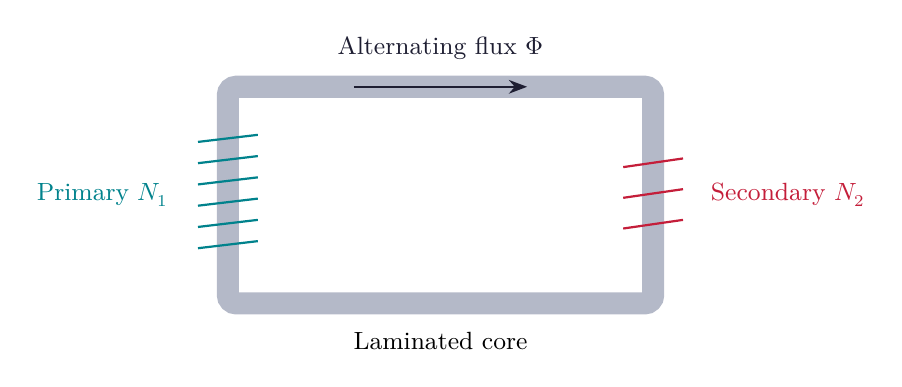
\begin{tikzpicture}[font=\small]
\draw[mgframe,line width=8pt,rounded corners=3pt] (0,0) rectangle (5.4,2.75);
\draw[-Stealth,mydark,thick] (1.6,2.75)--(3.8,2.75) node[midway,above=6pt] {Alternating flux $\Phi$};
\foreach \y in {0.7,0.97,1.24,1.51,1.78,2.05} {
  \draw[myteal,thick] (-0.38,\y)--(0.38,\y+0.09);
}
\foreach \y in {0.95,1.34,1.73} {
  \draw[myred,thick] (5.02,\y)--(5.78,\y+0.11);
}
\node[myteal,left=6pt] at (-0.42,1.38) {Primary $N_1$};
\node[myred,right=6pt] at (5.8,1.38) {Secondary $N_2$};
\node[below=7pt] at (2.7,0) {Laminated core};
\end{tikzpicture}
\end{tcolorbox}

For sinusoidal flux \(\Phi=\Phi_m\sin\omega t\), Faraday's law gives peak emf \(\omega N\Phi_m\). Hence
\[
\begin{aligned}
E_{\mathrm{rms}}&=\frac{2\pi fN\Phi_m}{\sqrt 2}\\
                &\approx 4.44 fN\Phi_m .
\end{aligned}
\]
Use \(f\) in hertz and peak flux in webers. For the ideal transformer, with \(a=N_1/N_2\), the magnitudes satisfy \(V_1/V_2=a\) and \(I_1/I_2=1/a\). An impedance on the secondary is referred to the primary as \(Z'_2=a^2Z_2\). Derive this by using \(V'_2=aV_2\) and \(I'_2=I_2/a\) in the impedance ratio.

\subsection{Equivalent circuit, losses and performance}
\begin{itemize}[leftmargin=*, itemsep=3pt, topsep=4pt]
  \item \textbf{Series elements.} Each winding has a resistance \(R_1\) or \(R_2\) for copper loss and a leakage reactance \(X_1\) or \(X_2\) for flux that links only that winding.
  \item \textbf{Shunt elements.} Across the induced primary emf, \(R_c\) represents core loss and \(jX_m\) represents the magnetising current.
  \item \textbf{Refer to the primary.} Multiply secondary impedance by \(a^2\), where \(a=N_1/N_2\). Hence \(R_{\mathrm{eq}}=R_1+a^2R_2\) and \(X_{\mathrm{eq}}=X_1+a^2X_2\).
  \item \textbf{Approximate circuit.} Move the shunt branch to the supply terminals. This neglects the small primary series drop due to no-load current.
\end{itemize}

\begin{tcolorbox}[tikzbox,title={Approximate equivalent circuit referred to the primary},unbreakable]
\centering
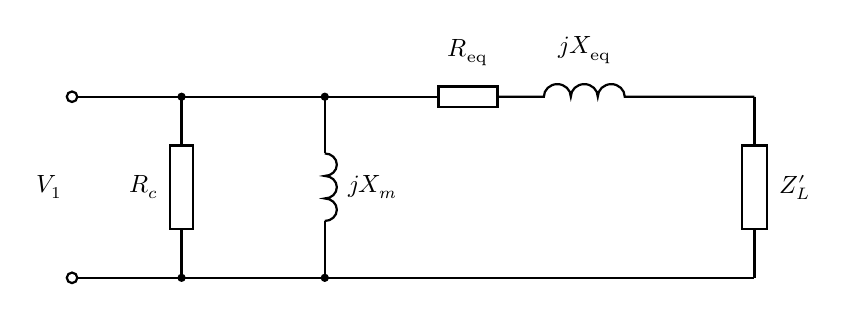
\begin{tikzpicture}[x=1.07cm,font=\small]
\draw[thick] (0,2.3)--(5.05,2.3) (0,0)--(8.1,0);
\draw[thick] (1.3,2.3)--(1.3,1.68) (1.3,0.62)--(1.3,0);
\draw[thick,fill=white] (1.16,0.62) rectangle (1.44,1.68);
\node[left] at (1.14,1.15) {$R_c$};
\draw[thick] (3.0,2.3)--(3.0,1.58) (3.0,0.72)--(3.0,0);
\draw[thick] (3.0,1.58) arc[start angle=90,end angle=-90,radius=0.143]
 arc[start angle=90,end angle=-90,radius=0.143]
 arc[start angle=90,end angle=-90,radius=0.143];
\node[right] at (3.16,1.15) {$jX_m$};
\draw[thick,fill=white] (4.35,2.17) rectangle (5.05,2.43);
\node[above=4pt] at (4.70,2.43) {$R_{\mathrm{eq}}$};
\draw[thick] (5.05,2.3)--(5.60,2.3)
 arc[start angle=180,end angle=0,radius=0.16]
 arc[start angle=180,end angle=0,radius=0.16]
 arc[start angle=180,end angle=0,radius=0.16] -- (8.1,2.3);
\node[above=4pt] at (6.09,2.46) {$jX_{\mathrm{eq}}$};
\draw[thick] (8.1,2.3)--(8.1,1.68) (8.1,0.62)--(8.1,0);
\draw[thick,fill=white] (7.95,0.62) rectangle (8.25,1.68);
\node[right] at (8.28,1.15) {$Z'_L$};
\node[left] at (0,1.15) {$V_1$};
\foreach \x in {1.3,3.0} {\fill (\x,2.3) circle (1.5pt); \fill (\x,0) circle (1.5pt);}
\draw[thick,fill=white] (0,0) circle (1.9pt) (0,2.3) circle (1.9pt);
\end{tikzpicture}
\end{tcolorbox}

\textbf{Losses to identify.}
\begin{itemize}[leftmargin=*, itemsep=3pt, topsep=4pt]
  \item \textbf{Core loss.} Hysteresis and eddy-current losses. Approximately constant at fixed supply voltage and frequency.
  \item \textbf{Copper loss.} \(I_1^2R_1+I_2^2R_2\). At load fraction \(x\), approximate it as \(x^2P_{\mathrm{cu,full}}\).
  \item \textbf{Other losses.} Stray load and dielectric losses also occur. The basic efficiency model below uses core and copper losses.
\end{itemize}

\textbf{Efficiency.} For a rating \(S_r\) in VA and load power factor \(\cos\phi\), output power is \(xS_r\cos\phi\) in W.
\[
\eta=\frac{xS_r\cos\phi}{xS_r\cos\phi+P_{\mathrm{core}}+x^2P_{\mathrm{cu,full}}}.
\]
Multiply \(\eta\) by 100 for percentage efficiency. At fixed positive power factor, maximising \(\eta\) is equivalent to minimising loss per unit of output. Apart from the constant \(1/(S_r\cos\phi)\), this gives
\[
\begin{aligned}
g(x)&=\frac{P_{\mathrm{core}}}{x}+xP_{\mathrm{cu,full}},\\
g'(x)&=-\frac{P_{\mathrm{core}}}{x^2}+P_{\mathrm{cu,full}},\\
g'(x)=0 &\quad\Longrightarrow\quad x^2P_{\mathrm{cu,full}}=P_{\mathrm{core}}.
\end{aligned}
\]
This is a minimum for \(x>0\) since \(g''(x)=2P_{\mathrm{core}}/x^3>0\). \textbf{Exam point.} At the optimum, the copper loss at that load equals the core loss.

Voltage regulation is the change in secondary terminal voltage from full load to no load with primary voltage held constant, divided by the full-load secondary voltage:
\[
\%\,\mathrm{reg}=\frac{V_{2,\mathrm{nl}}-V_{2,\mathrm{fl}}}{V_{2,\mathrm{fl}}}\times100 .
\]
\begin{itemize}[leftmargin=*, itemsep=3pt, topsep=4pt]
  \item \textbf{Lagging load.} For small voltage drops, approximate the numerator by \(I_2(R_{\mathrm{eq,2}}\cos\phi+X_{\mathrm{eq,2}}\sin\phi)\). All impedances here are referred to the secondary.
  \item \textbf{Leading load.} Use a minus sign for the reactance term. The no-load voltage can then be lower than the loaded voltage, giving negative regulation.
\end{itemize}

\begin{tcolorbox}[examplebox,title={Transformer performance at partial load}]
For a \(5\,\mathrm{kVA}\) transformer with \(60\,\mathrm W\) core loss and \(240\,\mathrm W\) full-load copper loss, take \(x=0.5\), \(\cos\phi=0.8\):
\[
\begin{aligned}
P_o&=(0.5)(5000)(0.8)=2000\,\mathrm W,\\
P_{\mathrm{cu}}&=(0.5)^2(240)=60\,\mathrm W,\\
\eta&=\frac{2000}{2000+60+60}=94.34\%.
\end{aligned}
\]
The core and copper losses are equal here, so this load fraction gives maximum efficiency at the same power factor.
\end{tcolorbox}

An \textbf{autotransformer} uses a tapped winding with a portion common to input and output. It transfers energy partly by conduction and partly by induction. For a ratio near unity it can save copper and reduce losses. The shared winding provides no galvanic isolation. Applications include voltage adjustment and reduced-voltage motor starting.

\subsection{DC machine construction and equations}
\begin{itemize}[leftmargin=*, itemsep=3pt, topsep=4pt]
  \item \textbf{Field system.} The stationary yoke and poles carry magnetic flux. Field windings or permanent magnets supply the excitation.
  \item \textbf{Armature.} A laminated rotor houses conductors in slots. The commutator connects the rotating conductors to stationary brushes.
  \item \textbf{Generator action.} The commutator switches coil connections so the voltage at the brushes is unidirectional.
  \item \textbf{Motor action.} As a coil crosses from one pole region to another, the commutator reverses its current to maintain the direction of torque.
\end{itemize}

For \(P\) poles, flux \(\Phi\) per pole in Wb, \(Z\) armature conductors, \(A\) parallel paths and speed \(N\) in rpm,
\[
\begin{aligned}
\text{flux swept per conductor per revolution}&=P\Phi,\\
\text{revolution time}&=60/N,\\
E&=\frac{P\Phi N}{60}\frac{Z}{A}.
\end{aligned}
\]
Neglect brush drop for the basic terminal equations:
\[
\begin{aligned}
V&=E-I_aR_a &&\text{generator supplying current},\\
V&=E_b+I_aR_a &&\text{motor drawing current}.
\end{aligned}
\]
In the motor, back emf \(E_b\) opposes the applied voltage. Divide the electromagnetic conversion power \(E_b I_a\) by \(\omega_m=2\pi N/60\) in rad/s to find torque.
\[
\begin{aligned}
T_e&=\frac{E_b I_a}{\omega_m}\\
   &=\frac{PZ}{2\pi A}\Phi I_a \quad(\mathrm{N\,m}).
\end{aligned}
\]
Shaft torque equals electromagnetic torque less the rotational-loss torque in motor operation.

\par\vspace{6pt}\noindent
\begin{tabularx}{\linewidth}{|B{3.4cm}|Y|Y|}\hline
Excitation & \textbf{Connection} & \textbf{Motor characteristic} \\ \hline
Separately excited & Field supplied externally. & Field and armature can be adjusted independently. \\ \hline
Shunt & Field across terminal supply. & Flux approximately constant, so speed changes moderately and torque is approximately proportional to \(I_a\). \\ \hline
Series & Field carries armature current. & Large starting torque, with torque approximately proportional to \(I_a^2\) before saturation. Speed can run high at light load. \\ \hline
Compound & Both shunt and series fields. & Cumulative compounding adds the two field effects and combines starting torque with better speed control than a series motor. \\ \hline
\end{tabularx}

\begin{itemize}[leftmargin=*, itemsep=3pt, topsep=4pt]
  \item \textbf{Shunt generator.} Terminal voltage droops under load because of the armature voltage drop and field and armature effects.
  \item \textbf{Series generator.} Voltage initially rises with load current. Magnetic saturation and internal drops limit that rise.
  \item \textbf{Compound generator.} Cumulative compounding adds series-field flux and can compensate terminal-voltage drop. Differential compounding subtracts series-field flux.
  \item \textbf{Motor speed.} For a given machine, \(N\) varies approximately as \((V-I_aR_a)/\Phi\). A series motor can overspeed at light load.
  \item \textbf{Starting.} At standstill \(N=0\) and \(E_b=0\), so the armature current would be high. A starter limits it using series resistance cut out in steps or electronic current limiting.
\end{itemize}

\begin{tcolorbox}[examplebox,title={DC motor back emf and converted torque}]
For \(V=220\,\mathrm V\), \(R_a=0.5\,\Omega\), \(I_a=20\,\mathrm A\) and \(N=1000\,\mathrm{rpm}\),
\[
\begin{aligned}
E_b&=220-(20)(0.5)=210\,\mathrm V,\\
P_{\mathrm{conv}}&=(210)(20)=4200\,\mathrm W,\\
T_e&=\frac{4200}{2\pi(1000)/60}=40.1\,\mathrm{N\,m}.
\end{aligned}
\]
\end{tcolorbox}

\subsection{AC motors, stepper motors and BLDC motors}
\begin{itemize}[leftmargin=*, itemsep=3pt, topsep=4pt]
  \item \textbf{Rotating field.} A balanced three-phase stator produces a field at \(N_s=120f/P\) rpm, with \(P\) poles and frequency \(f\) in Hz.
  \item \textbf{Induction motor.} Relative motion induces rotor current. That current interacts with the field to produce torque. A squirrel-cage rotor uses bars and end rings. A wound rotor can connect to external resistance through slip rings.
  \item \textbf{Synchronous motor.} The rotor field locks to the rotating stator field, so steady speed is \(N_s\).
\end{itemize}

In an induction motor, slip is \(s=(N_s-N_r)/N_s\), where \(N_r\) is rotor speed. Rotor electrical frequency is \(sf\). For a four-pole motor with \(f=50\,\mathrm{Hz}\) and \(N_r=1440\,\mathrm{rpm}\),
\[
\begin{aligned}
N_s &=120(50)/4=1500\,\mathrm{rpm},\\
s   &=(1500-1440)/1500=0.04,\\
sf  &=(0.04)(50)=2\,\mathrm{Hz}.
\end{aligned}
\]

\begin{tcolorbox}[tikzbox,title={From rotating field to induction-motor torque},unbreakable]
\centering
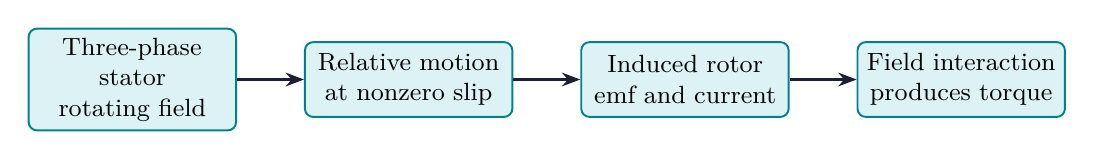
\begin{tikzpicture}[node distance=0.85cm,font=\small]
\node[block] (field) {Three-phase stator\\rotating field};
\node[block,right=of field] (slip) {Relative motion\\at nonzero slip};
\node[block,right=of slip] (current) {Induced rotor\\emf and current};
\node[block,right=of current] (torque) {Field interaction\\produces torque};
\draw[arrow] (field)--(slip);
\draw[arrow] (slip)--(current);
\draw[arrow] (current)--(torque);
\end{tikzpicture}
\end{tcolorbox}

\begin{itemize}[leftmargin=*, itemsep=3pt, topsep=4pt]
  \item \textbf{Main winding alone.} The pulsating field is equivalent to equal forward and backward rotating fields. Opposite torques cancel at standstill.
  \item \textbf{Starting methods.} Split-phase, capacitor-start and shaded-pole arrangements create a starting field asymmetry.
  \item \textbf{Applications.} Fans, pumps and domestic equipment.
\end{itemize}

\begin{itemize}[leftmargin=*, itemsep=3pt, topsep=4pt]
  \item \textbf{Stepper motor.} Sequential phase excitation advances the rotor in steps. A \(1.8^\circ\) motor takes \(360/1.8=200\) full steps per revolution. Indexing can use open-loop control within torque and speed limits. Feedback helps detect missed steps.
  \item \textbf{Brushless DC motor (BLDC).} A permanent-magnet rotor runs inside electronically commutated stator windings. The controller uses position sensing or sensorless estimation to switch phases. In automation, BLDC motors drive pumps, fans and servo axes.
\end{itemize}

\newpage
\begin{center}
  {\large\bfseries\color{myred} Quick Revision --- Module 4}\\[3pt]
  {\small\color{mydark} Transformers and Rotating Machines $|$ 26-ES-EE101}
\end{center}
\noindent{\color{myred}\rule{\linewidth}{1.2pt}}
\vspace{4pt}

\begin{tcolorbox}[formulabox, title={Key Formulas and Concepts at a Glance}]
\renewcommand{\arraystretch}{1.35}
\begin{tabularx}{\linewidth}{B{4.4cm}Y}
Transformer emf & $E=4.44fN\Phi_m$ in V for sinusoidal flux. \\[3pt]
Ideal turns ratio & $V_1/V_2=a$, $I_1/I_2=1/a$, $Z'_2=a^2Z_2$. \\[3pt]
DC emf and torque & $E=P\Phi ZN/(60A)$; $T_e=(PZ/2\pi A)\Phi I_a$. \\[3pt]
Speed and slip & $N_s=120f/P$ in rpm; $s=(N_s-N_r)/N_s$. \\[3pt]
\end{tabularx}
\end{tcolorbox}

\begin{tcolorbox}[defbox, title={One-Line Definitions}]
\textbf{Voltage regulation.} No-load to full-load voltage drop as a percentage of full-load voltage.

\textbf{Back emf.} Armature emf that opposes the applied voltage in a motor.

\textbf{Electronic commutation.} Timed switching of stator phases using a drive circuit.
\end{tcolorbox}

\begin{tcolorbox}[exambox, title={Frequently Asked / Viva Questions}]
\begin{enumerate}[topsep=0pt, label=\textbf{Q\arabic*.}, itemsep=5pt]
  \item \Q{Why laminate the core?} To limit circulating eddy currents and their losses.
  \item \Q{Why does transformer frequency stay the same?} The same alternating flux links the windings.
  \item \Q{What does the magnetising branch represent?} Core loss and current needed to establish flux.
  \item \Q{When is transformer efficiency maximum?} In the simple model at fixed power factor, when copper loss equals core loss.
  \item \Q{What is a main limitation of an autotransformer?} Its input and output are electrically connected through the common winding.
  \item \Q{What is the purpose of a motor starter?} It limits the large initial armature current while back emf is low.
  \item \Q{How does a series DC motor develop high starting torque?} Before saturation the flux rises with armature current, so torque is roughly proportional to $I_a^2$.
  \item \Q{Why is slip needed in an induction motor?} Relative motion induces rotor emf and develops torque.
  \item \Q{Why does a single-phase induction motor need a starting arrangement?} Its two opposing field components produce zero net starting torque with the main winding alone.
  \item \Q{How does a BLDC motor commutate?} An electronic controller switches the stator phases in sequence.
\end{enumerate}
\end{tcolorbox}

\begin{tcolorbox}[tikzbox, title={Summary Reference}]
\begin{tabularx}{\linewidth}{|B{4.0cm}|Y|}\hline
Topic & \textbf{What to remember} \\ \hline
Transformer & Static magnetic energy transfer with voltage conversion. \\ \hline
DC motor & Mechanical commutator and brushes switch armature current. \\ \hline
Induction motor & Rotor currents are induced by relative motion. \\ \hline
Stepper / BLDC & Discrete positioning / electronically commutated rotation. \\ \hline
\end{tabularx}
\end{tcolorbox}


% -- Module 5 -----------------------------------------------------------------
\modulestart{5}{Semiconductor Fundamentals and Diode Applications}

\section{Semiconductor Fundamentals and Diode Applications}

\subsection{Energy bands and semiconductor types}
\begin{tcolorbox}[defbox,title={Valence band, conduction band and band gap}]
The valence band contains the states associated with bonding electrons. Electrons in available conduction-band states can move through the solid and contribute to current. The band gap \(E_g\), measured in electronvolts (eV), separates these bands when there are no allowed states between them.
\end{tcolorbox}

\begin{itemize}[leftmargin=*, itemsep=3pt, topsep=4pt]
  \item \textbf{Conductor.} A partly filled band or overlapping bands provide nearby available states.
  \item \textbf{Insulator.} A wide gap leaves few thermally available carriers.
  \item \textbf{Semiconductor.} A smaller gap makes carrier density sensitive to temperature, doping and light.
  \item \textbf{Hole.} A missing electron in a nearly filled valence band behaves as a mobile positive charge.
\end{itemize}

\begin{tcolorbox}[tikzbox,title={Energy-band comparison},unbreakable]
\centering
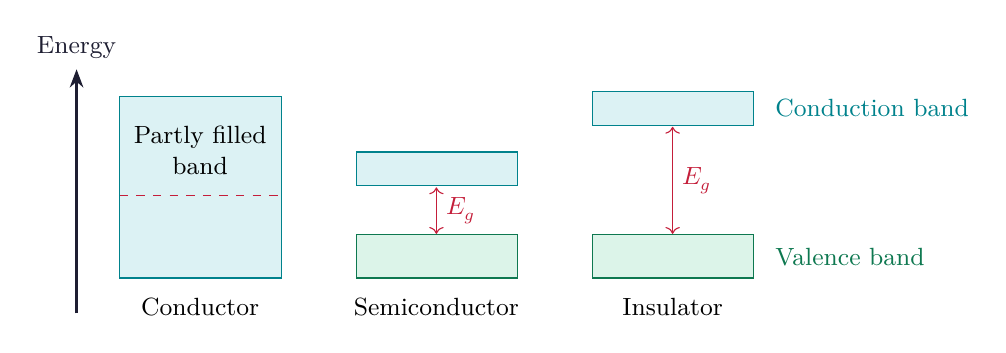
\begin{tikzpicture}[font=\small]
\draw[arrow] (-0.55,0.1)--(-0.55,3.2) node[above] {Energy};
\filldraw[fill=hdrteal,draw=myteal] (0,0.55) rectangle (2.05,2.85);
\draw[myred,dashed] (0,1.60)--(2.05,1.60);
\node[align=center] at (1.02,2.17) {Partly filled\\band};
\foreach \x/\gap in {3.00/0.62,6.00/1.39}{
  \filldraw[fill=hdrgreen,draw=mygreen] (\x,0.55) rectangle ++(2.05,0.55);
  \filldraw[fill=hdrteal,draw=myteal] (\x,{1.10+\gap}) rectangle ++(2.05,0.43);
  \draw[<->,myred] ({\x+1.02},1.11)--({\x+1.02},{1.08+\gap}) node[midway,right] {$E_g$};
}
\node[below] at (1.02,0.42) {Conductor};
\node[below] at (4.02,0.42) {Semiconductor};
\node[below] at (7.02,0.42) {Insulator};
\node[right,myteal] at (8.2,2.71) {Conduction band};
\node[right,mygreen] at (8.2,0.82) {Valence band};
\end{tikzpicture}
\end{tcolorbox}

\begin{itemize}[leftmargin=*, itemsep=3pt, topsep=4pt]
  \item \textbf{Intrinsic.} In undoped material, thermal generation creates electron--hole pairs. At equilibrium \(n=p=n_i\).
  \item \textbf{n-type extrinsic.} Donors such as phosphorus in silicon add available electrons. Electrons are the majority carriers.
  \item \textbf{p-type extrinsic.} Acceptors such as boron in silicon increase the hole concentration. Holes are the majority carriers.
  \item \textbf{Equilibrium check.} Minority carriers remain present and the bulk is electrically neutral. For nondegenerate material at equilibrium, \(np=n_i^2\).
\end{itemize}

\subsection{Drift and diffusion currents}
Drift is carrier motion due to an electric field. Electrons drift against the field and holes drift with the field. Both conventional drift current components point with the field. Diffusion is carrier motion from regions of higher carrier concentration towards lower concentration. In one dimension the conventional current densities are
\[
\begin{aligned}
J_n &= q n\mu_n E+q D_n \frac{dn}{dx},\\
J_p &= q p\mu_p E-q D_p \frac{dp}{dx}.
\end{aligned}
\]
Here \(q>0\) is the elementary charge in C, \(E\) is electric field in V/m, \(n,p\) are in \(\mathrm{m^{-3}}\), \(\mu\) is mobility in \(\mathrm{m^2/(V\,s)}\), \(D\) is diffusivity in \(\mathrm{m^2/s}\), and \(J\) is in \(\mathrm{A/m^2}\). The opposite diffusion signs come from electrons carrying negative charge. For uniform concentration conductivity is \(\sigma=q(n\mu_n+p\mu_p)\), in S/m.

\subsection{The p--n junction and diode characteristic}
\begin{tcolorbox}[defbox,title={Depletion region and bias}]
A p--n junction forms where p-type and n-type regions meet. Near the boundary, majority carriers diffuse and recombine, leaving exposed fixed ions. The resulting region has few mobile carriers and is called the depletion region. Forward bias connects the p-side to higher potential than the n-side. Reverse bias does the opposite.
\end{tcolorbox}

\begin{itemize}[leftmargin=*, itemsep=3pt, topsep=4pt]
  \item \textbf{At equilibrium.} Fixed ions produce a field from n-side to p-side. Diffusion and drift balance.
  \item \textbf{Forward bias.} Lower barrier and narrower depletion region allow strong carrier injection.
  \item \textbf{Reverse bias.} Higher barrier and wider depletion region limit current. Before breakdown the small reverse current is strongly temperature dependent.
\end{itemize}
\[
I_D=I_S\left(e^{V_D/(\eta V_T)}-1\right),\qquad V_T=\frac{kT}{q}\approx25.9\,\mathrm{mV}\quad(300\,\mathrm K).
\]
\(V_D\) is anode minus cathode voltage, \(I_D\) is positive from anode to cathode, \(I_S\) is reverse saturation current and \(\eta\) is the ideality factor. The exponential model applies before breakdown over the appropriate current range. A silicon diode drop of about \(0.7\,\mathrm V\) is an approximation for ordinary forward current, useful in circuit calculation. The bar on the schematic symbol marks the cathode.

\begin{tcolorbox}[tikzbox,title={Diode current--voltage characteristic (schematic)},unbreakable]
\centering
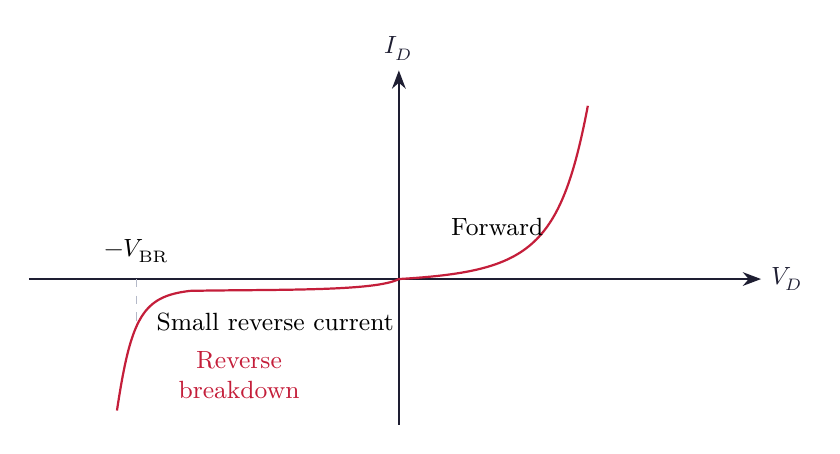
\begin{tikzpicture}[font=\small]
\draw[arrow] (-4.7,0)--(4.6,0) node[right] {$V_D$};
\draw[arrow] (0,-1.85)--(0,2.65) node[above] {$I_D$};
\draw[myred,thick] (-3.58,-1.67) .. controls (-3.40,-0.47) and (-3.25,-0.22) .. (-2.65,-0.15)
  .. controls (-1.6,-0.13) and (-0.3,-0.16) .. (0,0)
  .. controls (1.65,0.1) and (2.05,0.36) .. (2.4,2.2);
\draw[dashed,mgframe] (-3.33,0)--(-3.33,-0.59);
\node[above] at (-3.33,0.08) {$-V_{\mathrm{BR}}$};
\node[myred,align=center] at (-2.03,-1.22) {Reverse\\breakdown};
\node[above] at (1.25,0.43) {Forward};
\node[below] at (-1.57,-0.3) {Small reverse current};
\end{tikzpicture}
\end{tcolorbox}

\begin{itemize}[leftmargin=*, itemsep=3pt, topsep=4pt]
  \item \textbf{Zener breakdown.} Tunnelling through the narrow depletion region of a heavily doped junction.
  \item \textbf{Avalanche breakdown.} Impact ionisation creates more electron--hole pairs. It is favoured by a wider depletion region and generally higher breakdown voltage.
  \item \textbf{Practical point.} The mechanisms can coexist. Limit current to the device rating when using breakdown.
\end{itemize}

\subsection{Half-wave and full-wave rectifiers}
A \textbf{rectifier} converts an AC input into a unidirectional output. For a resistive load and ideal diodes:
\begin{itemize}[leftmargin=*, itemsep=3pt, topsep=4pt]
  \item \textbf{Half-wave.} One series diode conducts in one half cycle.
  \item \textbf{Centre-tapped full-wave.} Two diodes use alternate half-secondary windings. Load current has the same direction in both halves.
  \item \textbf{Bridge full-wave.} Four diodes use the full secondary. Two conduct per half cycle with the same load-current direction. Opposite corners receive AC. The common cathodes give the positive output and the common anodes the negative output.
\end{itemize}

\begin{tcolorbox}[tikzbox,title={Bridge rectifier and conducting paths},unbreakable]
\centering
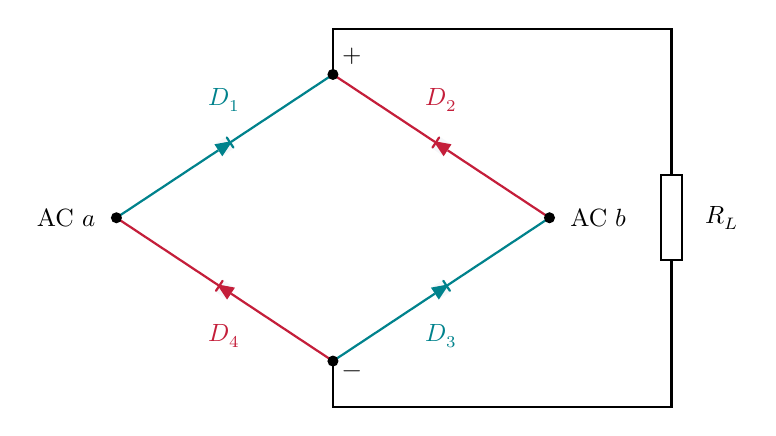
\begin{tikzpicture}[font=\small,line cap=round]
\coordinate (A) at (-2.75,0);
\coordinate (B) at (2.75,0);
\coordinate (P) at (0,1.82);
\coordinate (N) at (0,-1.82);
\foreach \from/\to/\lab/\clr/\side in {A/P/$D_1$/myteal/above,B/P/$D_2$/myred/above,N/B/$D_3$/myteal/below,N/A/$D_4$/myred/below}{
  \draw[thick,\clr] (\from)--(\to);
  \path (\from)--(\to) node[midway,sloped,allow upside down,fill=mygray,inner sep=0pt] {
    \tikz[baseline=-0.5ex,x=1em,y=1em]{
      \filldraw[fill=mygray,thick,\clr] (-0.32,-0.22)--(-0.32,0.22)--(0.20,0)--cycle;
      \draw[thick,\clr] (0.20,-0.24)--(0.20,0.24);
    }};
  \path (\from)--(\to) node[midway,\side=9pt,text=\clr] {\lab};
}
\draw[thick] (P)--(0,2.40)--(4.3,2.40)--(4.3,0.54)
  (4.3,-0.54)--(4.3,-2.40)--(0,-2.40)--(N);
\draw[thick,fill=white] (4.17,-0.54) rectangle (4.43,0.54);
\node[right=5pt] at (4.43,0) {$R_L$};
\fill (A) circle (2pt) (B) circle (2pt) (P) circle (2pt) (N) circle (2pt);
\node[left=4pt] at (A) {AC $a$};
\node[right=4pt] at (B) {AC $b$};
\node[above right] at (P) {$+$};
\node[below right] at (N) {$-$};
\end{tikzpicture}
\par\smallskip\small
\(a\) positive relative to \(b\): \(D_1,D_3\) conduct.
\quad \(b\) positive relative to \(a\): \(D_2,D_4\) conduct.
\end{tcolorbox}

\begin{tcolorbox}[tikzbox,title={Ideal unfiltered output waveforms},unbreakable]
\centering
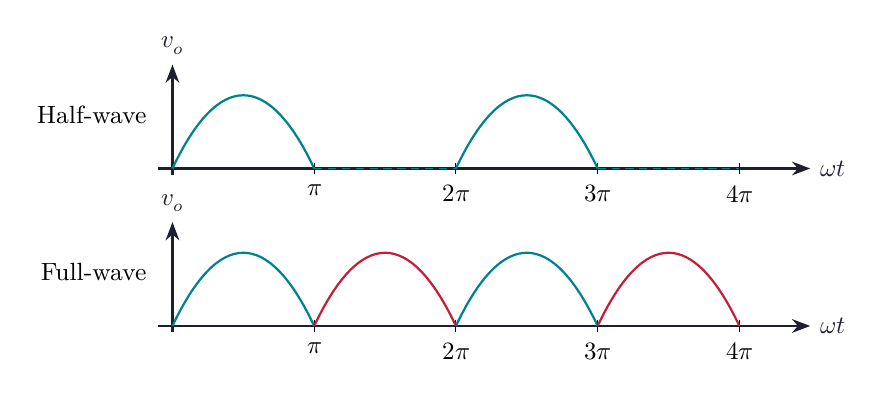
\begin{tikzpicture}[x=0.90cm,y=0.80cm,font=\small]
\foreach \y/\name in {2.5/Half-wave,0/Full-wave}{
  \node[left] at (-0.23,{\y+0.85}) {\name};
  \draw[arrow] (-0.2,\y)--(9.0,\y) node[right] {$\omega t$};
  \draw[arrow] (0,{\y-0.10})--(0,{\y+1.65}) node[above] {$v_o$};
  \foreach \x/\lab in {2/{\pi},4/{2\pi},6/{3\pi},8/{4\pi}}{
    \draw (\x,{\y-0.09})--(\x,{\y+0.09});
    \node[below] at (\x,{\y-0.11}) {$\lab$};
  }
  \foreach \x in {0,4}{
    \draw[myteal,thick] (\x,\y) .. controls ({\x+0.65},{\y+1.55})
    and ({\x+1.35},{\y+1.55}) .. ({\x+2},\y);
  }
}
\draw[myteal,thin,densely dashed] (2,2.5)--(4,2.5) (6,2.5)--(8,2.5);
\foreach \x in {2,6}{
  \draw[myred,thick] (\x,0) .. controls ({\x+0.65},1.55)
    and ({\x+1.35},1.55) .. ({\x+2},0);
}
\end{tikzpicture}
\end{tcolorbox}

For input frequency \(f\) and a peak output pulse \(V_m\) in the ideal unfiltered circuit,
\[
\begin{aligned}
V_{\mathrm{DC,half}}
 &=\frac{1}{2\pi}\int_0^\pi V_m\sin\theta\,d\theta
 =\frac{V_m}{\pi},\\
V_{\mathrm{DC,full}}
 &=\frac{2}{2\pi}\int_0^\pi V_m\sin\theta\,d\theta
 =\frac{2V_m}{\pi}.
\end{aligned}
\]
Supply the appropriate \(V_m\): in a centre-tapped design it is the peak of one half-secondary, and in a bridge it is the full-secondary peak. For the unfiltered ideal circuit the peak inverse voltage (PIV) per diode is \(V_m\) in half-wave and bridge circuits and \(2V_m\) in the centre-tapped circuit. A reservoir capacitor changes the off-state voltage in some topologies. With a real bridge take off approximately two forward drops from the peak.

\subsection{Filters and Zener voltage regulation}
A \textbf{filter} reduces AC ripple after rectification. A shunt capacitor charges near the peaks and supplies the load between them. For small ripple, approximate the discharge by \(\Delta Q=I_L/f_{\mathrm{ripple}}\). Since \(\Delta Q=C\Delta V\),
\[
\Delta V_{\mathrm{pp}}\approx\frac{I_L}{f_{\mathrm{ripple}}C},
\]
with \(f_{\mathrm{ripple}}=f\) for half-wave and \(2f\) for full-wave. The average filtered voltage is roughly the charged peak minus half the peak-to-peak ripple. An LC filter uses a series inductor to oppose ripple current and a shunt capacitor to bypass it. A capacitor--inductor--capacitor arrangement is called a \(\pi\) filter.

\begin{tcolorbox}[examplebox,title={Estimate the output from a filtered bridge}]
A \(12\,\mathrm{V}\) RMS, \(50\,\mathrm{Hz}\) secondary feeds a bridge with \(0.7\,\mathrm V\) per forward diode, \(C=1000\,\mu\mathrm F\) and \(I_L=0.10\,\mathrm A\).
\[
\begin{aligned}
V_{\mathrm{peak}}&\approx 12\sqrt2-2(0.7)=15.57\,\mathrm V,\\
\Delta V_{\mathrm{pp}}&\approx\frac{0.10}{100(1000\times10^{-6})}=1.00\,\mathrm V,\\
V_{\mathrm{DC}}&\approx15.57-\frac{1.00}{2}=15.07\,\mathrm V .
\end{aligned}
\]
\end{tcolorbox}

In a \textbf{Zener shunt regulator}, a series resistor \(R_S\) connects \(V_{\mathrm{in}}\) to the output. The reverse-biased Zener and load are in parallel, with the Zener cathode at the positive output. In breakdown \(V_o\approx V_Z\), and
\[
\begin{aligned}
I_S&=\frac{V_{\mathrm{in}}-V_Z}{R_S},\\
I_Z&=I_S-I_L,\qquad P_Z\approx V_Z I_Z .
\end{aligned}
\]
\begin{itemize}[leftmargin=*, itemsep=3pt, topsep=4pt]
  \item \textbf{Minimum current check.} Use minimum input voltage and maximum load current.
  \item \textbf{Maximum dissipation check.} Use maximum input voltage and minimum load current.
\end{itemize}
\begin{tcolorbox}[examplebox,title={Shunt-regulator current and power}]
For \(V_{\mathrm{in}}=12\,\mathrm V\), \(V_Z=5.1\,\mathrm V\), \(R_S=330\,\Omega\) and \(I_L=10\,\mathrm{mA}\),
\[
\begin{aligned}
I_S &= (12-5.1)/330 \approx20.91\,\mathrm{mA},\\
I_Z &= I_S-I_L \approx10.91\,\mathrm{mA},\\
P_Z &= V_Z I_Z \approx55.6\,\mathrm{mW}.
\end{aligned}
\]
\end{tcolorbox}

\subsection{Light-emitting diode and photodiode}
\begin{itemize}[leftmargin=*, itemsep=3pt, topsep=4pt]
  \item \textbf{Light-emitting diode (LED).} Forward-bias recombination emits photons. The material influences their energy \(hf\) and wavelength. Symbol arrows point outwards.
  \item \textbf{Current limiting.} Use a series resistor. For a \(5\,\mathrm V\) supply, a \(2\,\mathrm V\) LED and target \(10\,\mathrm{mA}\), \(R=(5-2)/0.01=300\,\Omega\).
  \item \textbf{Photodiode.} Incoming photons generate carriers. The depletion field separates them and gives a photocurrent proportional to light power in the linear region. Symbol arrows point inwards.
  \item \textbf{Bias and applications.} A photodiode can operate at zero bias or in reverse bias for a faster response. Dark current is the reverse current without light. Uses include optical links, light meters and sensors.
\end{itemize}



\newpage
\begin{center}
  {\large\bfseries\color{myred} Quick Revision --- Module 5}\\[3pt]
  {\small\color{mydark} Semiconductor Fundamentals and Diode Applications $|$ 26-ES-EE101}
\end{center}
\noindent{\color{myred}\rule{\linewidth}{1.2pt}}
\vspace{4pt}

\begin{tcolorbox}[formulabox, title={Key Formulas and Concepts at a Glance}]
\renewcommand{\arraystretch}{1.35}
\begin{tabularx}{\linewidth}{B{4.4cm}Y}
Thermal equilibrium & $np=n_i^2$; in intrinsic material $n=p=n_i$. \\[3pt]
Diode equation & $I_D=I_S[\exp(V_D/(\eta V_T))-1]$ before breakdown. \\[3pt]
Ideal mean rectifier output & $V_m/\pi$ for half-wave; $2V_m/\pi$ for full-wave. \\[3pt]
Capacitor ripple & $\Delta V_{\mathrm{pp}}\approx I_L/(f_{\mathrm{ripple}}C)$. \\[3pt]
Shunt regulation & $I_Z=(V_{\mathrm{in}}-V_Z)/R_S-I_L$. \\[3pt]
\end{tabularx}
\end{tcolorbox}

\begin{tcolorbox}[defbox, title={One-Line Definitions}]
\textbf{Band gap.} Energy interval without allowed states between the valence and conduction bands.

\textbf{Depletion region.} Junction region depleted of mobile carriers and containing exposed fixed ions.

\textbf{Ripple.} AC variation remaining on a rectified DC output.
\end{tcolorbox}

\begin{tcolorbox}[exambox, title={Frequently Asked / Viva Questions}]
\begin{enumerate}[topsep=0pt, label=\textbf{Q\arabic*.}, itemsep=5pt]
  \item \Q{What is a hole?} A missing valence-band electron that acts as a positive mobile carrier.
  \item \Q{What does a donor add?} A donor adds an available electron, increasing the electron concentration.
  \item \Q{How do drift and diffusion differ?} Drift is field-driven. Diffusion is driven by concentration gradients.
  \item \Q{What happens to the barrier in forward bias?} The applied voltage reduces the barrier and narrows the depletion region.
  \item \Q{What distinguishes Zener and avalanche breakdown?} Tunnelling versus impact ionisation.
  \item \Q{Why is a bridge full wave?} A different diode pair conducts each half cycle, maintaining the load-current direction.
  \item \Q{How does a reservoir capacitor reduce ripple?} It supplies load current between successive peaks.
  \item \Q{Which conditions give the largest Zener current?} Highest input voltage and lightest load, while the diode regulates.
  \item \Q{Why use an LED series resistor?} It limits current to the intended operating value.
  \item \Q{What is a photodiode's dark current?} Reverse current measured without optical illumination.
\end{enumerate}
\end{tcolorbox}

\begin{tcolorbox}[tikzbox, title={Summary Reference}]
\begin{tabularx}{\linewidth}{|B{4.0cm}|Y|}\hline
Topic & \textbf{What to remember} \\ \hline
Unfiltered half-wave & One pulse per supply cycle. \\ \hline
Unfiltered full-wave & Two pulses per supply cycle. \\ \hline
Filter and regulator & The filter reduces ripple. The regulator stabilises the output voltage. \\ \hline
LED and photodiode & The LED emits light. The photodiode senses it. \\ \hline
\end{tabularx}
\end{tcolorbox}


% -- Module 6 -----------------------------------------------------------------
\modulestart{6}{Transistors and Operational Amplifiers}

\section{Transistors and Operational Amplifiers}

\subsection{BJT structure, operation and bias modes}
\begin{tcolorbox}[defbox,title={Bipolar junction transistor}]
A bipolar junction transistor (BJT) is a three-terminal semiconductor device with emitter, base and collector regions arranged as NPN or PNP. A small base current can control a much larger collector current in forward-active operation. Both carrier types take part in device action.
\end{tcolorbox}

\begin{itemize}[leftmargin=*, itemsep=3pt, topsep=4pt]
  \item \textbf{Emitter.} Heavily doped to inject carriers into the base.
  \item \textbf{Base.} Thin and lightly doped so most carriers cross it with little recombination. Base current supplies recombination and injection into the emitter.
  \item \textbf{Collector.} Collects the carriers and handles reverse voltage and power.
\end{itemize}

\textbf{Forward-active operation.}
\begin{enumerate}[leftmargin=*, itemsep=3pt, topsep=4pt]
  \item In an NPN transistor, the base--emitter junction is forward biased and the base--collector junction is reverse biased.
  \item Electrons injected from the emitter diffuse across the thin base.
  \item The collector junction field sweeps most of them into the collector. PNP operation follows the same sequence with opposite polarities and holes as the main injected carriers.
\end{enumerate}

\begin{tcolorbox}[tikzbox,title={NPN and PNP transistor symbols},unbreakable]
\centering
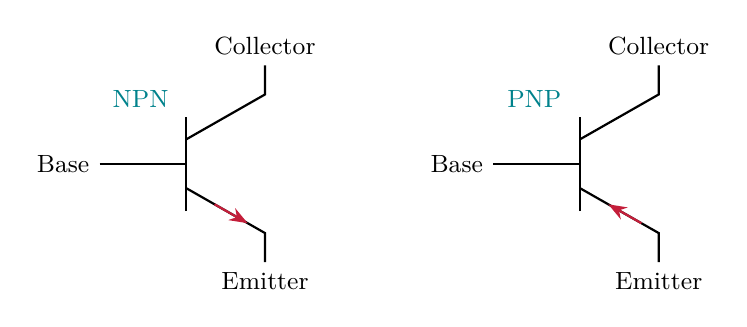
\begin{tikzpicture}[font=\small,line width=0.8pt]
\foreach \x/\name in {0/NPN,5.0/PNP}{
  \begin{scope}[shift={(\x,0)}]
  \draw (0,0)--(0,1.2) (-1.1,0.6)--(0,0.6);
  \draw (0,0.91)--(1.0,1.48)--(1.0,1.85);
  \draw (0,0.29)--(1.0,-0.28)--(1.0,-0.65);
  \node[left] at (-1.1,0.6) {Base};
  \node[above] at (1,1.85) {Collector};
  \node[below] at (1,-0.65) {Emitter};
  \node[myteal,above] at (-0.58,1.18) {\name};
  \end{scope}
}
\draw[-Stealth,myred,thick] (0.36,0.085)--(0.78,-0.155);
\draw[-Stealth,myred,thick] (5.78,-0.155)--(5.36,0.085);
\end{tikzpicture}
\end{tcolorbox}

\par\vspace{6pt}\noindent
\begin{tabularx}{\linewidth}{|B{3.3cm}|Y|Y|Y|}\hline
Region & \textbf{Emitter junction} & \textbf{Collector junction} & \textbf{Use or behaviour} \\ \hline
Cut-off & Reverse or effectively off & Reverse & Leakage only, switch open. \\ \hline
Forward active & Forward & Reverse & Current or voltage amplification. \\ \hline
Saturation & Forward & Forward & Switch on with small \(V_{CE}\). \\ \hline
Reverse active & Reverse & Forward & Roles are exchanged with reduced gain. \\ \hline
\end{tabularx}

For current magnitudes \(I_E=I_C+I_B\). Neglecting leakage in active operation,
\[
\begin{aligned}
\alpha&=\frac{I_C}{I_E},&
\beta&=\frac{I_C}{I_B},&
\gamma&=\frac{I_E}{I_B},\\
\beta&=\frac{I_C}{I_E-I_C}
      =\frac{\alpha}{1-\alpha},&
\alpha&=\frac{\beta}{1+\beta},&
\gamma&=1+\beta .
\end{aligned}
\]
\begin{itemize}[leftmargin=*, itemsep=3pt, topsep=4pt]
  \item \textbf{DC versus incremental gain.} DC ratios use the currents at one bias point. Incremental gains use small current changes around that point at fixed output voltage.
  \item \textbf{Check the operating mode.} Use \(I_C\approx\beta I_B\) in forward active operation. In saturation the external circuit mainly limits the collector current.
\end{itemize}

\subsection{CB, CE and CC characteristics}
\begin{itemize}[leftmargin=*, itemsep=3pt, topsep=4pt]
  \item \textbf{Common terminal.} This terminal belongs to both the input and output circuits.
  \item \textbf{Input characteristic.} Vary input voltage and record input current at a fixed output voltage.
  \item \textbf{Output characteristic.} Vary output voltage for a fixed input current. Repeat for different input currents. The table uses voltage magnitudes where convenient.
\end{itemize}
\par\vspace{6pt}\noindent
\begin{tabularx}{\linewidth}{|B{2cm}|Y|Y|Y|}\hline
Mode & \textbf{Input variables} & \textbf{Output variables} & \textbf{Gain and application} \\ \hline
CB & \(I_E,V_{BE}\) at fixed \(V_{CB}\). & \(I_C,V_{CB}\) at fixed \(I_E\). & Current gain \(\alpha<1\). Low input resistance. \\ \hline
CE & \(I_B,V_{BE}\) at fixed \(V_{CE}\). & \(I_C,V_{CE}\) at fixed \(I_B\). & Current gain \(\beta\). Resistively loaded voltage amplifier is inverting. \\ \hline
CC & \(I_B,V_{BC}\) at fixed \(V_{EC}\) for formal common-collector port variables. & \(I_E,V_{EC}\) at fixed \(I_B\). Voltage magnitudes may be plotted. & Current gain \(\gamma\). Emitter follower has nearly unity positive voltage gain and low output resistance. \\ \hline
\end{tabularx}

\begin{itemize}[leftmargin=*, itemsep=3pt, topsep=4pt]
  \item \textbf{Input curves.} CB and CE show a forward-junction shape in normal operation. In CC, \(V_{BE}=V_{BC}-V_{EC}\) relates the port voltage to the same junction.
  \item \textbf{CB and CC outputs.} In the active region \(I_C\approx\alpha I_E\) in CB and \(I_E\approx(1+\beta)I_B\) in CC. At fixed input current the output current changes only slightly with output voltage.
  \item \textbf{CE output.} Identify the low-voltage saturation knee, the active region with slight positive slope and the near-zero-base-current cut-off curve.
\end{itemize}

\begin{tcolorbox}[tikzbox,title={CE output characteristics and the Early effect},unbreakable]
\centering
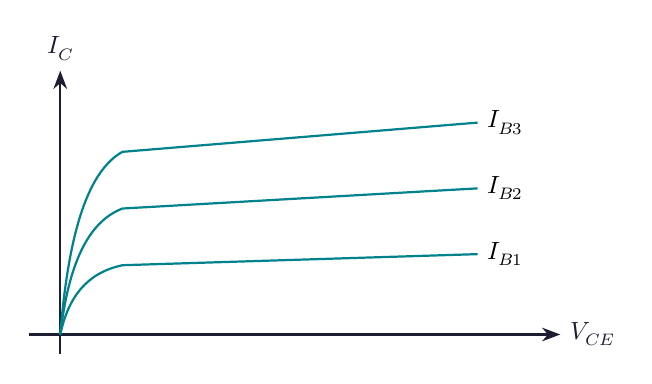
\begin{tikzpicture}[font=\small]
\draw[arrow] (-0.40,0)--(6.35,0) node[right] {$V_{CE}$};
\draw[arrow] (0,-0.25)--(0,3.35) node[above] {$I_C$};
\foreach \y/\lab in {0.88/1,1.60/2,2.32/3}{
  \draw[myteal,thick] (0,0) .. controls (0.10,{0.53*\y}) and (0.33,{0.89*\y})
  .. (0.79,\y) -- (5.3,{1.16*\y});
  \node[right] at (5.3,{1.16*\y}) {$I_{B\lab}$};
}
\end{tikzpicture}
\end{tcolorbox}

\begin{itemize}[leftmargin=*, itemsep=3pt, topsep=4pt]
  \item \textbf{Meaning.} The Early effect is modulation of the neutral base width.
  \item \textbf{Cause and effect.} Higher collector--base reverse bias narrows the neutral base, so collector current rises slightly in the active region.
  \item \textbf{Read the curve.} At fixed \(V_{BE}\), \(I_C\simeq I_{C0}(1+V_{CE}/V_A)\). Extend the active-region lines towards the voltage axis to estimate the intercept \(-V_A\). For \(V_A\gg V_{CE}\), the incremental output resistance is \(r_o\approx V_A/I_C\).
\end{itemize}

\subsection{Hybrid parameter model in outline}
The hybrid model is a linear two-port approximation for small signals near the DC bias (Q) point. It combines input resistance, reverse voltage ratio, forward current ratio and output admittance, giving it mixed units. For CE, use the port currents entering the device:
\[
\begin{aligned}
v_{be}&=h_{ie}i_b+h_{re}v_{ce},\\
i_c&=h_{fe}i_b+h_{oe}v_{ce}.
\end{aligned}
\]
\(h_{ie}\) (in \(\Omega\)) and \(h_{fe}\) (dimensionless) are found with the small-signal output voltage zero. \(h_{re}\) (dimensionless) and \(h_{oe}\) (in S) are found with the small-signal input current zero. These are incremental conditions about the Q point. In the unilateral approximation \(h_{re}\) is small. The output then looks like a controlled current \(h_{fe}i_b\) in parallel with \(1/h_{oe}\).

\begin{tcolorbox}[examplebox,title={Convert BJT current gains}]
For a transistor in forward active mode with \(\alpha=0.98\) and \(I_E=2\,\mathrm{mA}\),
\[
\begin{aligned}
\beta&=\frac{0.98}{1-0.98}=49,\\
I_C&=0.98(2)=1.96\,\mathrm{mA},\\
I_B&=2-1.96=0.04\,\mathrm{mA}=40\,\mu\mathrm A.
\end{aligned}
\]
\end{tcolorbox}

\subsection{Junction field-effect transistor}
\begin{tcolorbox}[defbox,title={JFET and pinch-off}]
A junction field-effect transistor (JFET) is a voltage-controlled device in which a reverse-biased gate junction changes the width of a conducting channel. Pinch-off at the drain end marks the start of the nearly constant drain-current region. Cut-off is the gate-bias condition where channel current becomes negligible.
\end{tcolorbox}

\begin{itemize}[leftmargin=*, itemsep=3pt, topsep=4pt]
  \item \textbf{Bias and symbol.} Use \(V_{DS}>0\) and \(V_{GS}\le 0\) for an n-channel JFET. Its reverse-biased gate draws very little current. The gate arrow points into an n-channel and out of a p-channel.
  \item \textbf{Common-source circuit.} Ground the source, connect \(R_D\) from the drain to \(V_{DD}\), and set the gate bias separately.
  \item \textbf{Drain characteristics.} Vary \(V_{DS}\) at fixed \(V_{GS}\) and record \(I_D\). Repeat at different gate voltages to obtain a family of curves.
\end{itemize}

\begin{tcolorbox}[tikzbox,title={N-channel JFET in a common-source circuit},unbreakable]
\centering
\begin{tikzpicture}[font=\small]
\draw[thick] (2.6,0)--(2.6,1.71) (2.6,2.06)--(2.6,2.76)
 (2.6,3.43)--(2.6,3.89);
\draw[thick,line width=1.5pt] (2.6,1.05)--(2.6,2.06);
\draw[-Stealth,thick,myteal] (0.35,1.56)--(2.6,1.56);
\draw[thick] (2.46,2.76) rectangle (2.74,3.43);
\draw[thick] (2.28,0)--(2.92,0) (2.37,-0.10)--(2.83,-0.10) (2.47,-0.20)--(2.73,-0.20);
\node[left] at (0.35,1.56) {$V_{GS}\le0$};
\node[above] at (2.6,3.89) {$V_{DD}$};
\node[right] at (2.76,3.09) {$R_D$};
\node[right] at (2.76,2.16) {Drain};
\node[right] at (2.76,0.72) {Source};
\end{tikzpicture}
\end{tcolorbox}

At small \(V_{DS}\) the channel is nearly ohmic. Increasing \(V_{DS}\) widens its depletion region near the drain. Beyond the boundary \(V_{DS}\approx V_{GS}-V_P\), with \(V_P=V_{GS(\mathrm{off})}<0\), the drain current is nearly constant until breakdown. More negative gate voltage lowers the whole curve. The transfer characteristic in the saturation region is approximately
\[
I_D=I_{DSS}\left(1-\frac{V_{GS}}{V_P}\right)^2,\qquad V_P\le V_{GS}\le0 .
\]
Here \(I_{DSS}\) is the saturation drain current at \(V_{GS}=0\). For \(I_{DSS}=8\,\mathrm{mA}\), \(V_P=-4\,\mathrm V\) and \(V_{GS}=-2\,\mathrm V\), \(I_D=8(1-0.5)^2=2\,\mathrm{mA}\). This solution requires \(V_{DS}\gtrsim2\,\mathrm V\) and below breakdown.

\subsection{MOSFET construction and output characteristics}
\begin{itemize}[leftmargin=*, itemsep=3pt, topsep=4pt]
  \item \textbf{Definition.} A metal--oxide--semiconductor field-effect transistor (MOSFET) uses an insulated gate to control the channel.
  \item \textbf{Construction.} An n-channel enhancement device has \(n^+\) source and drain regions in a p-type body. A thin insulator separates gate and body. Many discrete devices tie the body to the source.
  \item \textbf{Enhancement action.} Positive \(V_{GS}\) above the model threshold \(V_{TH}\) induces an inversion channel. A p-channel device uses opposite polarities and carrier types.
  \item \textbf{Depletion device.} It has a channel at \(V_{GS}=0\). Gate bias can reduce or increase channel conduction.
\end{itemize}

For a long-channel n-channel enhancement device with body tied to source, ignore subthreshold conduction and channel-length modulation. Define \(V_{\mathrm{ov}}=V_{GS}-V_{TH}\) and \(k_n=\mu_n C_{\mathrm{ox}}W/L\) in \(\mathrm{A/V^2}\). Then
\[
I_D=
\begin{cases}
0,& V_{GS}\le V_{TH},\\
k_n\bigl(V_{\mathrm{ov}}V_{DS}-V_{DS}^2/2\bigr),
   &0\le V_{DS}<V_{\mathrm{ov}},\\
k_n V_{\mathrm{ov}}^2/2,& V_{DS}\ge V_{\mathrm{ov}}>0 .
\end{cases}
\]
\begin{itemize}[leftmargin=*, itemsep=3pt, topsep=4pt]
  \item \textbf{Read the curve.} Each \(I_D\)--\(V_{DS}\) curve rises in the ohmic or triode region, reaches a knee at \(V_{DS}=V_{\mathrm{ov}}\) and flattens in saturation. A higher \(V_{GS}\) increases both the plateau current and knee voltage.
  \item \textbf{Choose the region.} Amplifiers normally bias a MOSFET in saturation. A fully enhanced switch operates in the low-resistance ohmic region. Real saturation curves slope upward slightly, and BJT saturation is a different bias condition.
\end{itemize}

\begin{tcolorbox}[tikzbox,title={FET drain characteristics (schematic)},unbreakable]
\centering
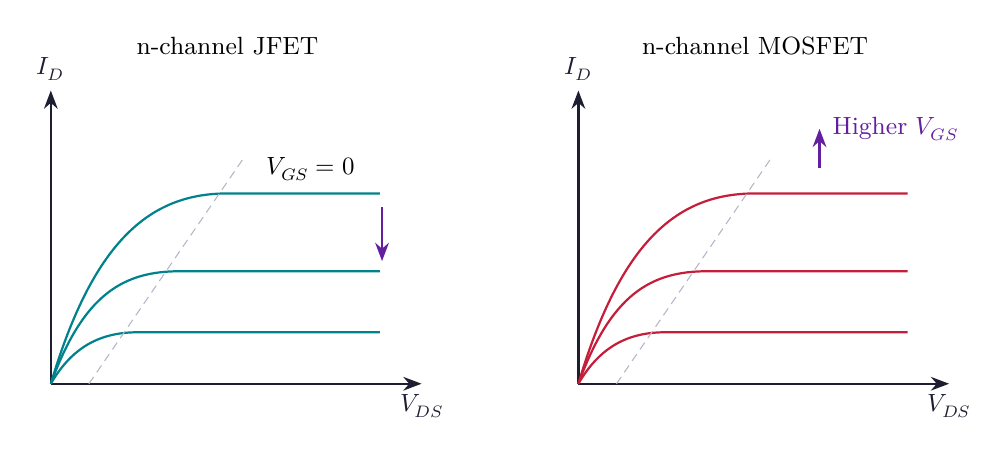
\begin{tikzpicture}[x=0.88cm,y=0.76cm,font=\small]
\begin{scope}
\draw[arrow] (0,0)--(5.35,0) node[below] {$V_{DS}$};
\draw[arrow] (0,0)--(0,4.90) node[above] {$I_D$};
\node[above] at (2.55,5.33) {n-channel JFET};
\draw[myteal,thick] (0,0) .. controls (0.62,2.42) and (1.45,3.18) .. (2.55,3.18)--(4.75,3.18);
\draw[myteal,thick] (0,0) .. controls (0.47,1.50) and (1.05,1.88) .. (1.86,1.88)--(4.75,1.88);
\draw[myteal,thick] (0,0) .. controls (0.30,0.60) and (0.70,0.86) .. (1.25,0.86)--(4.75,0.86);
\draw[densely dashed,mgframe] (0.55,0)--(2.80,3.80);
\node[above] at (3.75,3.22) {$V_{GS}=0$};
\draw[-Stealth,mypurple,thick] (4.78,2.95)--(4.78,2.05);
\end{scope}
\begin{scope}[xshift=6.7cm]
\draw[arrow] (0,0)--(5.35,0) node[below] {$V_{DS}$};
\draw[arrow] (0,0)--(0,4.90) node[above] {$I_D$};
\node[above] at (2.55,5.33) {n-channel MOSFET};
\draw[myred,thick] (0,0) .. controls (0.62,2.42) and (1.45,3.18) .. (2.55,3.18)--(4.75,3.18);
\draw[myred,thick] (0,0) .. controls (0.47,1.50) and (1.05,1.88) .. (1.86,1.88)--(4.75,1.88);
\draw[myred,thick] (0,0) .. controls (0.30,0.60) and (0.70,0.86) .. (1.25,0.86)--(4.75,0.86);
\draw[densely dashed,mgframe] (0.55,0)--(2.80,3.80);
\draw[-Stealth,mypurple,thick] (3.48,3.60)--(3.48,4.26) node[right=1pt] {Higher $V_{GS}$};
\end{scope}
\end{tikzpicture}
\par\smallskip\small
Dashed lines mark the transition into saturation. The JFET arrow points towards more negative \(V_{GS}\). The MOSFET shown is an enhancement device.
\end{tcolorbox}

\subsection{Op-amp model, open-loop response and parameters}
\begin{tcolorbox}[defbox,title={Operational amplifier}]
An op-amp is a high-gain differential voltage amplifier. It amplifies \(v_+-v_-\) and ideally rejects voltage common to both inputs. Negative feedback makes the closed-loop gain depend primarily on an external network.
\end{tcolorbox}

\begin{itemize}[leftmargin=*, itemsep=3pt, topsep=4pt]
  \item \textbf{Open-loop voltage response.} For small differential voltage, \(v_o=A_{\mathrm{OL}}(v_+-v_-)\). The steep transfer curve levels off at the positive and negative output swing limits.
  \item \textbf{Frequency response.} With a dominant pole, \(\lvert A_{\mathrm{OL}}\rvert\) is nearly flat at low frequency and falls at about \(20\,\mathrm{dB}\) per decade beyond the pole.
  \item \textbf{Ideal model.} Infinite open-loop gain, input resistance and bandwidth. Zero output resistance and offset. Perfect common-mode and supply rejection.
  \item \textbf{Use in circuit problems.} With stable negative feedback and linear operation, take \(i_+=i_-=0\) and \(v_+\approx v_-\). Check input range, output swing and slew rate before using these approximations.
\end{itemize}

\begin{itemize}[leftmargin=*, itemsep=3pt, topsep=4pt]
  \item \textbf{Input offset and bias.} Offset voltage is the differential voltage required for zero output. Bias current is the average of the input currents.
  \item \textbf{Gain-bandwidth product.} Approximately constant for a single dominant pole.
  \item \textbf{Slew rate.} Maximum output slope in V/\(\mu\)s. For a sinusoid with peak \(V_m\) and frequency \(f\), require \(\mathrm{SR}\ge 2\pi f V_m\), using consistent time units.
  \item \textbf{Rejection ratios.} \(\mathrm{CMRR}=20\log_{10}\lvert A_d/A_{\mathrm{cm}}\rvert\) in dB measures rejection of common-mode inputs. Supply rejection measures sensitivity to supply changes.
\end{itemize}

\subsection{Inverting, non-inverting, summing and difference amplifiers}
\begin{tcolorbox}[tikzbox,title={Inverting amplifier with negative feedback},unbreakable]
\centering
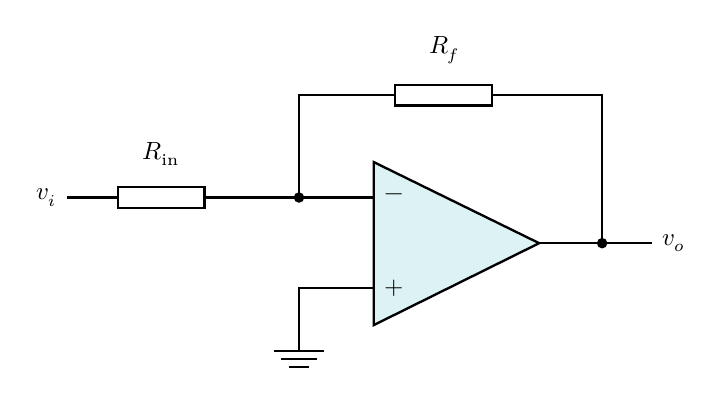
\begin{tikzpicture}[font=\small,line width=0.85pt]
\draw[fill=hdrteal] (4.25,0.08)--(4.25,2.15)--(6.35,1.12)--cycle;
\node at (4.51,1.70) {$-$};
\node at (4.51,0.55) {$+$};
\draw (0.36,1.70)--(1.0,1.70) (2.1,1.70)--(4.25,1.70);
\draw (1.0,1.57) rectangle (2.1,1.83);
\node[above=4pt] at (1.55,1.83) {$R_{\mathrm{in}}$};
\draw (3.30,1.70)--(3.30,3.00)--(4.52,3.00)
 (5.75,3.00)--(7.15,3.00)--(7.15,1.12);
\draw (4.52,2.87) rectangle (5.75,3.13);
\node[above=4pt] at (5.14,3.13) {$R_f$};
\draw (4.25,0.55)--(3.30,0.55)--(3.30,-0.25);
\draw (2.98,-0.25)--(3.62,-0.25) (3.07,-0.35)--(3.53,-0.35) (3.17,-0.45)--(3.43,-0.45);
\draw (6.35,1.12)--(7.78,1.12);
\fill (3.30,1.70) circle (1.9pt) (7.15,1.12) circle (1.9pt);
\node[left] at (0.36,1.70) {$v_i$};
\node[right] at (7.78,1.12) {$v_o$};
\end{tikzpicture}
\end{tcolorbox}

For the \textbf{inverting amplifier}, the non-inverting input is grounded. The inverting input is at virtual ground and draws negligible current. KCL at that node gives
\[
\begin{aligned}
\frac{v_i-0}{R_{\mathrm{in}}}&=\frac{0-v_o}{R_f},\\
v_o&=-\frac{R_f}{R_{\mathrm{in}}}v_i.
\end{aligned}
\]
For the \textbf{non-inverting amplifier}, \(v_+=v_i\). Connect \(R_g\) from the inverting node to ground and \(R_f\) from output to that node:
\[
\begin{aligned}
v_-&=\frac{R_g}{R_g+R_f}v_o,\\
v_o&=\left(1+\frac{R_f}{R_g}\right)v_i .
\end{aligned}
\]
Direct negative feedback gives a unity-gain voltage follower with high input resistance and low output resistance.

For an \textbf{inverting summer}, several voltages \(v_k\) feed the virtual-earth node through separate resistors \(R_k\). KCL adds the currents, giving \(v_o=-R_f\sum_k v_k/R_k\). With equal input resistors the circuit gives a scaled sum.

For a \textbf{difference amplifier}, connect \(v_1\) through \(R_1\) to the inverting node, \(R_2\) from output to that node, \(v_2\) through \(R_3\) to the non-inverting node and \(R_4\) from that node to ground. Then
\[
\begin{aligned}
v_+ &= \frac{R_4}{R_3+R_4}v_2,\\
\frac{v_1-v_+}{R_1}&=\frac{v_+-v_o}{R_2},\\
v_o&=\left(1+\frac{R_2}{R_1}\right)
      \frac{R_4}{R_3+R_4}v_2-\frac{R_2}{R_1}v_1.
\end{aligned}
\]
When \(R_2/R_1=R_4/R_3=k\), this reduces to \(v_o=k(v_2-v_1)\). Resistor-ratio mismatch gives some common-mode gain.

\begin{tcolorbox}[examplebox,title={Closed-loop gain and output swing}]
An inverting amplifier has \(R_{\mathrm{in}}=10\,\mathrm{k}\Omega\), \(R_f=47\,\mathrm{k}\Omega\), and practical output limits of \(\pm 10\,\mathrm V\).
\[
\begin{aligned}
A_v&=-\frac{47}{10}=-4.7,\\
v_o&=(-4.7)(0.8)=-3.76\,\mathrm V .
\end{aligned}
\]
A \(3\,\mathrm V\) input would require \(-14.1\,\mathrm V\), so the output instead clips near the negative limit and the virtual-ground relation no longer applies. For the matched difference-amplifier ratios \(k=4.7\), \(v_1=0.4\,\mathrm V\) and \(v_2=0.8\,\mathrm V\), the linear output is \(4.7(0.8-0.4)=1.88\,\mathrm V\).
\end{tcolorbox}

\newpage
\begin{center}
  {\large\bfseries\color{myred} Quick Revision --- Module 6}\\[3pt]
  {\small\color{mydark} Transistors and Operational Amplifiers $|$ 26-ES-EE101}
\end{center}
\noindent{\color{myred}\rule{\linewidth}{1.2pt}}
\vspace{4pt}

\begin{tcolorbox}[formulabox, title={Key Formulas and Concepts at a Glance}]
\renewcommand{\arraystretch}{1.35}
\begin{tabularx}{\linewidth}{B{4.4cm}Y}
BJT current ratios & $\beta=\alpha/(1-\alpha)$; $\gamma=1+\beta$. \\[3pt]
JFET saturation current & $I_D=I_{DSS}(1-V_{GS}/V_P)^2$ in its valid bias range. \\[3pt]
Op-amp voltage gains & $-R_f/R_{\mathrm{in}}$ (inverting); $1+R_f/R_g$ (non-inverting). \\[3pt]
Matched difference amplifier & $v_o=(R_2/R_1)(v_2-v_1)$. \\[3pt]
Inverting summer & $v_o=-R_f\sum_k v_k/R_k$. \\[3pt]
\end{tabularx}
\end{tcolorbox}

\begin{tcolorbox}[defbox, title={One-Line Definitions}]
\textbf{Early effect.} Change of collector current with collector voltage due to modulation of the neutral base width.

\textbf{Transconductance.} Incremental change in output current per unit input voltage.

\textbf{Virtual short.} Nearly equal op-amp input voltages under linear negative feedback.

\textbf{Slew rate.} Maximum rate at which an amplifier output voltage can change.
\end{tcolorbox}

\begin{tcolorbox}[exambox, title={Frequently Asked / Viva Questions}]
\begin{enumerate}[topsep=0pt, label=\textbf{Q\arabic*.}, itemsep=5pt]
  \item \Q{Why is the BJT base thin?} Most injected carriers cross it before recombining.
  \item \Q{Which junctions are forward biased in BJT saturation?} Both emitter--base and collector--base junctions.
  \item \Q{What gain does the common-collector connection give?} It gives current gain $\gamma=1+\beta$ and approximately unity voltage gain.
  \item \Q{What causes the slope of CE active characteristics?} The Early effect from base-width modulation.
  \item \Q{Why are h-parameters called hybrid?} Their units include ohms, siemens and dimensionless ratios.
  \item \Q{Does JFET pinch-off mean zero drain current?} Pinch-off starts current saturation. Gate cut-off is the near-zero-current condition.
  \item \Q{What forms the enhancement MOSFET channel?} Gate bias above threshold induces a conducting inversion layer.
  \item \Q{When can we equate the op-amp input voltages?} With high gain, stable negative feedback and linear operation.
  \item \Q{What determines an inverting amplifier gain?} The resistor ratio $-R_f/R_{\mathrm{in}}$.
  \item \Q{When does a difference amplifier reject common-mode input?} When the resistor ratios match and the op-amp is within its linear limits.
  \item \Q{What does slew rate limit?} Maximum output slope and therefore large-signal response at high frequency.
\end{enumerate}
\end{tcolorbox}

\begin{tcolorbox}[tikzbox, title={Summary Reference}]
\begin{tabularx}{\linewidth}{|B{4.0cm}|Y|}\hline
Topic & \textbf{What to remember} \\ \hline
BJT & Base controls collector current. Check active or saturated bias. \\ \hline
JFET and MOSFET & A reverse-biased junction or insulated gate controls a conducting channel. \\ \hline
Op-amp & Show the feedback connection, apply KCL, then test the output swing. \\ \hline
\end{tabularx}
\end{tcolorbox}


\end{document}
